     Armstrong relations are critical to the results developed in this
paper.  While the main example of this paper is the granule logic
developed in Sec.\ \ref{sec:setting}, many of the fundamental
underpinnings are in fact completely independent of this example, and
hold in a very general context.  They are in fact, easier, not more
difficult, to develop in a general context.  In this section, some of
those properties are developed.
    \par
     By far, the most comprehensive study of Armstrong models is
\mycite{Fagin82}, to which the reader is referred for a thorough
presentation of that subject in a general context.  In this section,
only the ideas critical to this work are developed.


 \begin{metalabpara}{summary}{}
         {Summary of Armstrong models}\envlabel{summ:armstrong}
       Let $\logicsys{L}$ be a logical system.  A set
 $\armctxt{C} \subseteq \wffof{L}$ is said to \emph{admit Armstrong
models} if for any satisfiable $\Phi \subseteq \armctxt{C}$, there is an
$M \in \modelsof{\Phi}$ with the property that for any
 $\varphi \in \armctxt{C}$, $M \in \modelsof{\varphi}$ iff
 $\Phi \sentails \varphi$.
    In other words, for any $\Phi \subseteq \armctxt{C}$, there is a
model which satisfies only those sentences of $\armctxt{C}$ which are
consequences of those in $\Phi$, and no others.
 \end{metalabpara}


 \begin{metalabpara}{myexample}{}
         {Armstrong models in granule logic}\envlabel{ex:armgran}
    In the context of this paper, the important case is
  $\armctxt{C} = \pbinconstrgrsch{G}$.  While it follows easily from
the more general result of \mycite[3.18]{HegnerRo17_inform} that
$\pbinconstrgrsch{G}$ admits Armstrong models, a much stronger result
is established in Sec. \ref{sec:pinfrules}.  Specifically, it is shown
how to construct an Armstrong model, called the canonical model, for
$\pconstrgrsch{G}$.  Since $\granschemaname{G}$ is arbitrary, this is
essentially equivalent to showing how to construct an Armstrong model
for any $\Phi \subseteq \pbinconstrgrsch{G}$.  That model will serve
as the foundation for developing crucial properties of the inference
systems developed in this paper.
 \end{metalabpara}


 \begin{metaemphlabpara}{corollary}{Corollary}
         {The canonical structure is a model of all of
the constraints}\envlabel{cor:canmodel}
   If $\constrgrsch{G}$ is satisfiable, then 
   $\canstrname{G} \in \modelsof{\constrgrsch{G}}$.
 \begin{proof}
  Assume that $\constrgrsch{G}$ is satisfiable.  For every
 $\varphi \in \pbinconstrgrsch{G}$, $\canstrname{G}$ is a model of
either $\varphi$ or else of $\mlnot\varphi$, but never both.
  Since $\canstrname{G}$ is a model of only those
 $\varphi \in \pbinconstrgrsch{G}$ for which
 $\pconstrgrsch{G} \sentails \varphi$,
 it must be model of all
 $\mlnot\varphi$ for which
 $\pconstrgrsch{G} \not\sentails \varphi$
 (see \envref{thm:canmodel}).
 Since all $\mlnot\varphi \in \nconstrgrsch{G}$ have this latter
property, it follows that $\canstrname{G}$ is a model of
$\nconstrgrsch{G}$, whence it is a model of all of $\constrgrsch{G}$.
 \end{proof}
 \end{metaemphlabpara}



with $k \geq 2$,
 for $g_1, g_2 \in \granulesofsch{G}$, then
 $\pconstrgrsch{G} \sentails \subrulep{g_1}{g_2}$.
    Put another way, if there is $k \in \natnum$ with
 $k \geq 2$ and $g_1', g_2', \ldots, g_k' \in \granulesof{G}$
 with $g_1 \ideq g_1'$, $g_2 \ideq g_k'$ and
    $\subrulep{g_i'}{g_{i+1}'} \in \pconstrgrsch{G}$
 for all $i \in \natint{1}{k-1}$,
 then $\pconstrgrsch{G} \sentails \subrulep{g_1}{g_2}$.


\begin{metalabpara}{mydefinition}{}
         {Subsumption-safe schemata}\envlabel{def:subsafesch}
    In any granule structure $\sigma$, it is always the case that
 \preformat{\linebreak}
 $\gnletodom{\sigma}(\botgrsch{G})=\emptyset$, while for no
 $g \in \granulesofschnb{G}$ is it the case that
 $\gnletodom{\sigma}(g)
 \preformat{\linebreak}
 = \emptyset$.
 Consequently, a constraint of the form $\subrulep{g}{\botgrsch{G}}$
is never satisfiable.
    Formally, call the schema $\granschemaname{G}$ \emph{subsumption
safe} if for no $g \in \granulesofschnb{G}$ is it the case that
 $\subrulep{g}{\botgrsch{G}} \in \pconstrgrsch{G}$.
   Alternatively, it is easy to see that $\granschemaname{G}$ is
subsumption safe iff for no $g \in \granulesofschnb{G}$ is it the case
that
 $\sgrpr{g}{\botgrsch{G}} \in \sgedgesstarofgrsch{G}$.
 \end{metalabpara}


 \begin{metalabpara}{mydefinition}{}
        {Single-use proofs}\envlabel{def:single}
    It may be the case that an antecedent of a proof is used several
times.  For example, in the proof shown in 
 (\ref{def:single}-1) below, the formula $\subrulep{g_3}{g_4}$
is used twice, once in $d_1$ and once in $d_2$.
 \[
    \tag{\ref{def:single}-1}
    \begin{prooftree}
     \hypoii{\subrulep{g_3}{g_4}}
            {\subrulep{g_4}{g_1}}
     \inferi[d_1]{\subrulep{g_3}{g_1}}
     \hypoii{\subrulep{g_3}{g_4}}
            {\subrulep{g_4}{g_2}}
     \inferi[d_2]{\subrulep{g_3}{g_2}}
     \hypoi{\disjrule{g_1}{g_2}}
     \inferiii[d_3]{\false}
    \end{prooftree}
 \]
  Call such a proof \emph{multiple use}.  On the other hand, call
proofs in which each antecedent occurrence is a distinct formula, such
as those in (\ref{def:rulenot}-1) and (\ref{def:rulenot}-2),
\emph{single use}, since they use each antecedent only once.
     \par
   Call a proof system \emph{single use} if for any set
 $\setbr{\alpha_1,\alpha_2,\ldots,\alpha_k}$ of formulas, and any
single formula $\beta$, if there is a proof of $\beta$ from 
 $\setbr{\alpha_1,\alpha_2,\ldots,\alpha_k}$, then there is a
single-use proof.
     \par
   It is worth noting now that even though the proof of 
(\ref{def:single}-1) is multiple use, it is possible to prove
$\false$ from
   $\setbr{\subrulep{g_3}{g_4},
           \subrulep{g_4}{g_1},
           \subrulep{g_4}{g_2},
           \disjrulep{g_1}{g_2}}$
 with a single-use proof.  Indeed, such a proof is possible using only
one rule instance, as shown in (\ref{def:single}-2) below.
 \[
    \tag{\ref{def:single}-2}
    \begin{prooftreem}
     \hypoiii{\subrulep{g_4}{g_1}}
             {\subrulep{g_4}{g_2}}
             {\disjrule{g_1}{g_2}}
     \inferi{\false}
    \end{prooftreem}
 \]
   It is not necessary to use $\subrulep{g_3}{g_4}$ in the
proof.  The proof systems developed in this paper for granule rules
are all single use, as will be established later.
     \par
   The idea of ``using up'' formulas, without permitting their re-use,
was introduced by Girard in the context of \emph{linear logic}
\mycite{Girard95_all}.
   Since it is not central to the results of this paper, linear logic
will not be considered further.
 \end{metalabpara}




Combined, these two constitute, in effect, a proof that
   $\grpr{\setbr{g_1,g_2}}{\setbr{g_1',g_2'}}
      \in \sgedgesstarofgrschii{G}$.
    The disjointness assertion $\disjrulep{g_1'}{g_2'}$ to the right
is assumed to be already in $\pconstrgrsch{G}$.  The conclusion
$\disjrulep{g_1}{g_2}$ must hold because it is a protected pair
according to \envref{def:protected}, and it is precisely such pairs
which are required to be disjoint by $\pconstrgrsch{G}$.  Since this
form of proof can deduce all valid protected pairs, it is complete for
disjointness rules.


    Call $\armctxt{C} \subseteq \wffof{L}$ \emph{complement free} if
for no $\varphi \in \armctxt{C}$ is there a
 $\varphi' \in \armctxt{C}$
 with the property that $\mlnot\varphi$ is equivalent to $\varphi'$,
in the precise sense that both $\mlnot\varphi \sentails \varphi'$ and
$\varphi' \sentails \mlnot\varphi$ hold.


 \begin{metalabpara}{context}{}
         {Context for this section}\envlabel{ctxt:armstrong}
     Throughout this section, unless stated specifically to the
contrary, take $\logicsys{L}$ be a logical system with the compactness
property, and let
  $\armctxt{C} \subseteq \wffof{L}$ be a nonempty set of sentences which
admits Armstrong models.
     Furthermore, take $\proofsys{A}$ to be a sound proof system which is
complete for $\armctxt{C}$.
 \end{metalabpara}



 \begin{metaemphlabpara}{lemma}{Lemma}
    {Entailment and satisfiability
                    in an Armstrong setting}\envlabel{lem:infposc}
     Let $\Phi$ be an extended Armstrong constraint set over
$\armctxt{C}$,
 and let $\beta \in \armctxt{C}$.
   \baxblkc
     \axitem{(a)} If $\Phi$ is satisfiable and $\Phi \sentails \beta$,
  then it must be the case that $\posof{\Phi} \sentails \beta$.
     \axitem{(b)} If $\Phi$ is satisfiable and
 $\Phi \sentails \mlnot\beta$,
 then either $\posof{\Phi} \sentails \mlnot\beta$, or else there is
 a $\mlnot\varphi \in \negof{\Phi}$ with the property that
    $\posof{\Phi} \union \setbr{\mlnot\varphi} \sentails \mlnot\beta$
 (and hence
    $\posof{\Phi} \union \setbr{\beta} \sentails \varphi$)
 holds,  with both $\posof{\Phi} \union \setbr{\mlnot\varphi}$ and
   $\posof{\Phi} \union \setbr{\beta}$ satisfiable.
    \axitem{(c)} If $\Phi$ is not satisfiable, then either
$\posof{\Phi}$ is unsatisfiable or else there is a
 $\mlnot\varphi \in \negof{\Phi}$ with
 $\posof{\Phi} \union \setbr{\mlnot\varphi}$ unsatisfiable.
  \eaxblk
  \begin{proof}
    Part (a): Assume that $\Phi$ is satisfiable with
 $\Phi \sentails \beta$.
 If $\Phi = \posof{\Phi}$, then there is nothing further to prove.
So, assume that there is a $\mlnot\varphi \in \negof{\Phi}$, and let
$M$ be an Armstrong model for $\posof{\Phi}$.  It cannot be the case
that
 $\posof{\Phi} \sentails \varphi$,
 for if it were to hold, then applying
\envref{lem:genswap}(a$'$),
  $\posof{\Phi} \union \setbr{\mlnot\varphi}$ would have to be
unsatisfiable, in contradiction to the satisfiability of $\Phi$.
    Since $M$ is an Armstrong model of $\posof{\Phi}$ and
 $\posof{\Phi} \not\sentails \varphi$, $M$ is a model of
$\mlnot\varphi$, and since $\mlnot\varphi$ was chosen arbitrarily from
$\negof{\Phi}$, $M$ is a model of all of $\Phi$.  Since $\Phi
\sentails \beta$, it follows that $M$ is also a model of $\beta$,
whence, by the definition of Armstrong model, $\posof{\Phi} \sentails
\beta$.
     \par
    Part (b): Assume that $\Phi$ is satisfiable with
 $\Phi \sentails \mlnot\beta$.  Using the compactness theorem
\envref{summ:compactness}(b), there is a finite subset $\Phi_o
\subseteq \Phi$ with $\Phi_0 \sentails \mlnot\beta$.
    Let $\Phi_0' \subseteq \Phi_0$ be a minimal subset of $\Phi_0$
with the property that $\Phi_0' \sentails \mlnot\beta$, in the sense
that for any proper subset $\Phi_0'' \subsetneq \Phi_0'$,
 $\Phi_0'' \not\sentails \mlnot\beta$.
    If $\Phi_o' \subseteq \posof{\Phi}$, there is nothing further to
prove.  So, assume that there is a $\mlnot\varphi \in \negof{\Phi_0'}$.
 Then since
  $(\Phi_0' \setminus \setbr{\mlnot\varphi})
         \union \setbr{\mlnot\varphi} \sentails \mlnot\beta$,
 an application of \envref{lem:genswap}(a) yields
     $(\Phi_0' \setminus \setbr{\mlnot\varphi})
                \union \setbr{\beta}  \sentails \varphi$.
  Furthermore, since $\Phi_o'$ is minimal,
  $\Phi_0' \setminus \setbr{\mlnot\varphi}
           \sentails \mlnot\beta$
  cannot hold, whence
  $(\Phi_0' \setminus \setbr{\mlnot\varphi}) \union \setbr{\beta}$
  is satisfiable by \envref{lem:genswap}(b).
  Invoking (a) on
     $(\Phi_0' \setminus \setbr{\mlnot\varphi})
                \union \setbr{\beta}  \sentails \varphi$,
 it follows that 
     $\posof{\Phi_0'} \union \setbr{\beta}  \sentails \varphi$,
 and so \emph{a fortiori},
     $\posof{\Phi} \union \setbr{\beta}  \sentails \varphi$.
  A second application of \envref{lem:genswap}(a) yields
     $\posof{\Phi} \union \setbr{\mlnot\varphi} \sentails \mlnot\beta$,
 as required.
   \par
 Part (c): Assume that $\Phi$ is not satisfiable.  Then, using
\envref{summ:compactness}(b), there is a finite subset
 $\Phi_0 \subseteq \Phi$ which is also unsatisfiable.  Without loss of
generality, choose $\Phi_0$ to be minimal in the sense that all of its
proper subsets are satisfiable.  If $\Phi_0 = \posof{\Phi_0}$, then
since $\posof{\Phi_0} \subseteq \posof{\Phi}$, $\posof{\Phi}$ is
unsatisfiable, and there is nothing more to prove.  So, assume that
 $\negof{\Phi_0} \neq \emptyset$, and let
 $\mlnot\varphi \in \negof{\Phi_0}$.  Then, since
 $\Phi_0 = (\Phi_0 \setminus \setbr{\mlnot\varphi})
                                 \union \setbr{\varphi}$
 is unsatisfiable, it follows from \envref{lem:genswap}(a$'$) that
 $\Phi_0 \sentails \varphi$.  Note furthermore that
 $\Phi_0 \setminus \setbr{\mlnot\varphi}$
 is satisfiable, since $\Phi_0$ is minimal unsatisfiable in the sense
described above, and that $\varphi \in \armctxt{C}$, just by
construction.  Thus, invoking (a),
 $\posof{\Phi_0 \setminus \setbr{\mlnot\varphi}}
   \sentails \varphi$,
 and since
  $\posof{\Phi_0} = \posof{\Phi_0 \setminus \setbr{\mlnot\varphi}}$,
 it follows that $\posof{\Phi_0} \sentails \varphi$.
 Finally, using \envref{lem:genswap}(a$'$) once again,
 $\posof{\Phi_0} \union \setbr{\mlnot\varphi}$ is unsatisfiable, and
since $\posof{\Phi_0} \subseteq \posof{\Phi}$,
  $\posof{\Phi} \union \setbr{\mlnot\varphi}$ is also unsatisfiable,
completing the proof.
  \end{proof}
 \end{metaemphlabpara}


   \parvert
   The next lemma, which is established in the context of an extended
Armstrong constraint set $\Phi$, is central to the results of this section.
     Part (a) asserts that if a positive assertion $\beta$ is a
consequence of $\Phi$, then it is a consequence of just the positive
assertions in $\Phi$.  In other words, negative assertions play no
r{\^o}le in establishing positive results.
     Part (b) asserts that if a negative assertion $\mlnot\beta$ is a
consequence of $\Phi$, then it is a consequence of the positive
assertions in $\Phi$ plus at most one of its negative assertions.  In
other words, establishing a negative assertions requires the use of at
most one other negative assertion.
     Finally, part (c) identifies the special case of (b) in which the
conclusion $\mlnot\beta$ is unsatisfiable.


 \begin{metalabpara}{summary}{}
         {Summary of compactness}\envlabel{summ:compactness}
    The \emph{compactness theorem} is a fundamental result of
propositional and first-order logic.  In its most fundamental form, it
may be expressed as follows (see \mycite[Thm.\ 11.22]{Monk76} or
\mycite[pp.\ 59--60]{Enderton01_book}).
   \baxblkc
      \axitem{(a)} {\slshape For $\Phi \subseteq \wffof{L}$, if every
finite subset $\Phi_0 \subseteq \Phi$ has a model, then so too does
$\Phi$ itself.}
   \eaxblk
     It has many equivalent ways of expression, including the
following (see \mycite[Cor.\ 17A]{Enderton01_book}).
   \baxblkc
     \axitem{(b)} {\slshape If $\Phi \subseteq \wffof{L}$ and
 $\varphi \in \wffof{L}$, then $\Phi \sentails \varphi$ iff
 $\Phi_0 \sentails \varphi$ for some finite subset
 $\Phi_0 \subseteq \Phi$.}
   \eaxblk
     Although it does not hold for an arbitrary logic, this result
does hold for all propositional and first-order logics.  Granule logic
is essentially propositional, so it holds in that logic in particular.
   \par
    Say that a logic $\logicsys{L}$ has the \emph{compactness
property} if (a) (or, equivalently (b)) above holds in that logic.
 \end{metalabpara}


 \begin{metalabpara}{context}{}
         {Context extension --- compactness}\envlabel{ctxt:compact}
     For the rest of this section, unless stated specifically to the
contrary, in addition to the conditions given in
\envref{ctxt:armctxt}, assume that $\logicsys{L}$ has the compactness
property.
 \end{metalabpara}


 \begin{metalabpara}{myexample}{Example}
         {The canonical Armstrong model for
            $\emptyset\subseteq\pbinconstrgrsch{G}$}\envlabel{ex:canarm}
     It is interesting to examine the canonical Armstrong model (see
\envref{def:canstr} and \envref{thm:canmodel}) for
$\constrgrsch{G}=\emptyset$.
    The canonical structure $\canstrdef{G}$ has $\candomgrsch{G}$ as
defined in \envref{def:canstr}, with
   $\fn{\canfngrsch{G}}{\granulesofsch{G}}{\powerset{\candomgrsch{G}}}$
 defined by
   $\canfngrsch{G}(g) = \setbr{\cangrelt{g}} \union
    \setdef{\cangrset{S} \in \doubletsofgrsch{G}}{g \in S}$
 for $g \in \granulesofsch{G}$, and
   $\canfngrsch{G}{\botgrsch{G}} = \emptyset$.
   The first part, $\setbr{\cangrelt{g}}$ arises from the application
of (canfn-i), while the second part,
    $\setdef{\cangrset{S} \in \doubletsofgrsch{G}}{g \in S}$,
 arises from the application of (canfn-ii), since all pairs are
unprotected.  The operation (canfn-iii) is never used since there are
no subsumption constraints.
 \end{metalabpara}


The main application of the general result of \envref{lem:cparm} is
with
 $\wffset{A} = \allarm{\armctxt{C}}$,
 and in the main example with
 $\wffset{A} = \allbinconstrgrsch{G}$.


 \begin{metalabpara}{discussion}{Discussion and examples}
    {Entailment in extended Armstrong constraint sets}\envlabel{disc:entarm}
   The results of \envref{prop:entarm} provide the key to extending an
inference system over $\armctxt{C}$ to one over
$\allarm{\armctxt{C}}$.
   \par
   Examine part (a) of \envref{prop:entarm} xxxxx.
   \par
   Examine part (b) of \envref{prop:entarm} xxxxx.
 \end{metalabpara}


  \parvert
    It is also possible to develop the negative binary tautologies,
but since they are not necessary for this work, the topic is not
pursued further.


    It is shown that the combined rules of Figs.\ \ref{fig:infrulespmain}
and \ref{fig:infrulesn} are consistent and sat-conditional complete
for inference on the two binary constraints of subsumption and
disjointness. as well as their negations.
    \par
    Technically, the four tautology rules on the bottom row of
Fig.\ \ref{fig:infrulesp} should also be swapped, with the resulting
rules deducing $\false$.  Rather than taking that approach, it is
shown that a set of positive and negative constraints is unsatisfiable
if one of the negations of the consequent of these rules; that is,
one of $\nsubrulep{g}{g}$, $\nsubrulep{g}{\top}$,
$\nsubrulep{\bot}{g}$, or $\ndisjrulep{\bot}{g}$ may be derived for
some granule $g$.  Together with the characterization of positive
unsatisfiability given above (derivation of one of assertions
$\subrulep{g}{\bot}$, $\disjrulep{g}{g}$ for some $g$ other than
$\bot$), these six cases constitute a complete set for deducing
unsatisfiability.
     \par


 \begin{metaemphlabpara}{proposition}{Proposition}
         {Consistency of swapping}\envlabel{prop:genswap}
    Let $\proofsys{A}$ be a proof system on $\wffset{A}$, and suppose
further that $\wffset{A}$ is closed under complements.
    If
    \[
    \begin{prooftree}
     \hypoi{\alpha_1~~\alpha_2~~\ldots~~\alpha_{k-1}~~\alpha_k}
     \inferi{\beta}
    \end{prooftree}
    \]
 is a consistent and minimal inference rule of $\proofsys{A}$, then
   \[
    \begin{prooftree}
     \hypoi{\alpha_1~~\alpha_2~~\ldots~~\alpha_{k-1}~~\mlnot\beta}
     \inferi{\mlnot\alpha_k}
    \end{prooftree}
    \]
  is also a consistent and minimal inference rule.
   In particular, if
    \[
    \begin{prooftree}
     \hypoi{\alpha_1~~\alpha_2~~\ldots~~\alpha_{k-1}~~\alpha_k}
     \inferi{\false}
    \end{prooftree}
    \]
 is a valid inference rule of $\proofsys{A}$ on $\wffset{A}$, then so
too is
   \[
    \begin{prooftree}
     \hypoi{\alpha_1~~\alpha_2~~\ldots~~\alpha_{k-1}}
     \inferi{\mlnot\alpha_k}
    \end{prooftree}
    \]
   \begin{proof}
      The proof follows directly from \envref{lem:genswap}.
   \end{proof}
 \end{metaemphlabpara}


     \par
     In order to deliver full completeness, it is necessary to apply
special swap operations to obtain unsatisfiability rules.  Looking
first at the rules of Fig.\ \ref{fig:infrulespmain}, there are two
ways to do this.  In the first, imagine an additional $\true$ premise
for each rule, and swap that premise with the conclusion, negating
each.  The result is shown in Fig.\ \ref{fig:infrulespmainunsat}.

  \begin{figure}[htb]
   \begin{gather*}
    \begin{prooftreem}
      \hypoi{\subrulep{\granvar{g}_1}{\granvar{g}_2} \hspace*{1cm}
             \subrulep{\granvar{g}_2}{\granvar{g}_3} \hspace*{1cm}
             \nsubrulep{\granvar{g}_1}{\granvar{g}_3}}
      \inferi{\false}
    \end{prooftreem} \\[1.25em]
   \begin{prooftreem}
     \hypoi{\subrulep{\granvar{g}_1'}{\granvar{g}_1} \hspace*{1cm}
            \subrulep{\granvar{g}_2'}{\granvar{g}_2} \hspace*{1cm}
            \disjrulep{\granvar{g}_1}{\granvar{g}_2} \hspace*{1cm}
            \ndisjrulep{\granvar{g}_1'}{\granvar{g}_2'}}
     \inferi{\false}
    \end{prooftreem}
   \end{gather*}
  \caption{Swapped main unsatisfiability rules for binary constraints ii}\label{fig:infrulespmainunsat}
  \end{figure}

   In the second, which is shown in
Fig.\ \ref{fig:infrulespmainunsatalt} and is perhaps simpler, xxxxx.

  \begin{figure}[htb]
   \begin{align*}
    \begin{prooftreem}
      \hypoi{\subrulep{\granvar{g}_1}{\granvar{g}_2} \hspace*{1cm}
             \nsubrulep{\granvar{g}_1}{\granvar{g}_2}}
      \inferi{\false}
    \end{prooftreem}
   &&
   \begin{prooftreem}
     \hypoi{\disjrulep{\granvar{g}_1}{\granvar{g}_2} \hspace*{1cm}
            \ndisjrulep{\granvar{g}_1'}{\granvar{g}_2'}}
     \inferi{\false}
    \end{prooftreem}
   \end{align*}
  \caption{Alternate swapped main unsatisfiability rules for binary constraints ii}\label{fig:infrulespmainunsatalt}
  \end{figure}

  \begin{figure}[htb]
  \belowdisplayskip=0em
    \begin{align*}
    \begin{prooftreem}
      \hypoi{\phantom{X}}
      \inferi{\nsubrulep{\granvar{g}}{\bot}}
    \end{prooftreem}
    {\scriptstyle\abr{|{\scriptscriptstyle(\granvar{g} \neq \bot)}}}
    &&
    \begin{prooftreem}
      \hypoi{\phantom{X}}
      \inferi{\ndisjrulep{\granvar{g}}{\granvar{g}}}
    \end{prooftreem}
    {\scriptstyle\abr{|{\scriptscriptstyle(\granvar{g} \neq \bot)}}}
   \end{align*}
  \caption{Swapped unsatisfiability rules for binary constraints}\label{fig:infrulespcontrswap}
  \end{figure}

  \begin{figure}[htb]
  \belowdisplayskip=0em
    \begin{align*}
    \begin{prooftreem}
      \hypoi{\nsubrulep{\granvar{g}}{\granvar{g}}}
      \inferi{\false}
    \end{prooftreem}
    &&
    \begin{prooftreem}
      \hypoi{\nsubrulep{\granvar{g}}{\top}}
      \inferi{\false}
    \end{prooftreem}
    &&
    \begin{prooftreem}
      \hypoi{\nsubrulep{\bot}{\granvar{g}}}
      \inferi{\false}
    \end{prooftreem}
    &&
    \begin{prooftreem}
      \hypoi{\ndisjrulep{\bot}{\granvar{g}}}
      \inferi{\false}
    \end{prooftreem}
   \end{align*}
  \caption{Swapped tautology rules for binary constraints}\label{fig:infrulesptautswap}
  \end{figure}

 Similarly, Figs.\ \ref{fig:infrulesptautswap} and
\ref{fig:infrulespcontrswap} show the swapped versions of the rules of
Figs.\ \ref{fig:infrulesptaut} and \ref{fig:infrulespcontr},
respectively.  Note in particular that the tautology rules of
Fig.\ \ref{fig:infrulesptaut} become unsatisfiability rules under swap
in Fig.\ \ref{fig:infrulesptautswap} and, conversely, the
unsatisfiability rules of Fig.\ \ref{fig:infrulespcontr} become
tautology rules under swap in Fig.\ \ref{fig:infrulespcontrswap}.


    If $k=0$; \ie, if
  $\setdef{\alpha_i}{i \in \ccinterval{1}{k}} = \emptyset$, then think
of the rule as having a single antecedent $\true$, which becomes
$\false$ upon negation.  The transformaion is thus
    \begin{align*}
    \tag{\ref{def:ruleswap}-3}
    \begin{prooftreem}
     \hypoi{\phantom{\true}}
     \inferi{\beta}
    \end{prooftreem}
    \hspace*{1cm} \equiv \hspace*{1cm}
    \begin{prooftreem}
     \hypoi{\true}
     \inferi{\beta}
    \end{prooftreem}
    \transto{\sepval}
    \begin{prooftreem}
     \hypoi{\mlnot\beta}
     \inferi{\mlnot\true}
    \end{prooftreem}
    \hspace*{1cm} \equiv \hspace*{1cm}
    \begin{prooftreem}
     \hypoi{\mlnot\beta}
     \inferi{\false}
    \end{prooftreem}
    \end{align*}


 \begin{metalabpara}{myexample}{}
      {The swap closure of $\bininfpos{G}$}\envlabel{def:swapclpbininf}
   Upon applying the construction of \envref{def:ruleswap}(b) to the
rules of $\bininfpos{G}$, a new inference system, denoted
 $\bininf{G}$, is obtained.
   Its rules are defined by 
    $\infrulesof{\bininf{G}} =
      \infrulesof{\swapcl{\bininfpos{G}}}$.
    \par
     More precisely, in addition to the eight rules
(pbinf-i)--(pbinf-viii), as defined in \ref{def:pbinf}, it includes the
following ten additional rules, with the way in which each rule was
obtained via swapping shown to its far right.
    \par\noindent
   \baxblke
     \axitem{(pbinf-i-sa)}
   $\begin{prooftreem}
      \hypoii{\subrulep{\granvar{g}_1}{\granvar{g}_2}}
             {\nsubrulep{\granvar{g}_1}{\granvar{g}_3}}
      \inferi{\nsubrulep{\granvar{g}_2}{\granvar{g}_3}}
      \end{prooftreem}$
      \hfill ($\rswap{\text{(pbinf-i)}}{\subrulep{\granvar{g}_2}{\granvar{g}_3}}$)
     \axitem{(pbinf-i-sb)}
   $\begin{prooftreem}
      \hypoii{\subrulep{\granvar{g}_2}{\granvar{g}_3}}
             {\nsubrulep{\granvar{g}_1}{\granvar{g}_3}}
      \inferi{\nsubrulep{\granvar{g}_1}{\granvar{g}_2}}
     \end{prooftreem}$
      \hfill ($\rswap{\text{(pbinf-i)}}{\subrulep{\granvar{g}_1}{\granvar{g}_2}}$)
     \axitem{(pbinf-ii-sa)}
   $\begin{prooftreem}
     \hypoiii{\subrulep{\granvar{g}_1}{\granvar{g}_1'}}
             {\subrulep{\granvar{g}_2}{\granvar{g}_2'}}
             {\ndisjrulep{\granvar{g}_1}{\granvar{g}_2}}
     \inferi{\ndisjrulep{\granvar{g}_1'}{\granvar{g}_2'}}
    \end{prooftreem}$
      \nlrightt ($\rswap{\text{(pbinf-ii)}}{\disjrulep{\granvar{g}_1'}{\granvar{g}_2'}}$)
     \axitem{(pbinf-ii-sb)}
   $\begin{prooftreem}
      \hypoiii{\ndisjrulep{\granvar{g}_1}{\granvar{g}_2}}
              {\subrulep{\granvar{g}_2}{\granvar{g}_2'}}
              {\disjrulep{\granvar{g}_1'}{\granvar{g}_2'}}
      \inferi{\nsubrulep{\granvar{g}_1}{\granvar{g}_1'}}
    \end{prooftreem}$
      \nlrightt ($\rswap{\text{(pbinf-ii)}}{\subrulep{\granvar{g}_1}{\granvar{g}_1'}}$)
      \axitem{(pbinf-iii-s)}
    \begin{prooftreem}
      \hypoi{\nsubrulep{\granvar{g}}{\granvar{g}}}
      \inferi{\false}
    \end{prooftreem}
     \hfill ($\rswap{\text{(pbinf-iii)}}{\true}$)
      \axitem{(pbinf-iv-s)}
    \begin{prooftreem}
      \hypoi{\nsubrulep{\granvar{g}}{\topgrsch{G}}}
      \inferi{\false}
    \end{prooftreem}
     \hfill ($\rswap{\text{(pbinf-iv)}}{\true}$)
      \axitem{(pbinf-v-s)}
    \begin{prooftreem}
      \hypoi{\nsubrulep{\botgrsch{G}}{\granvar{g}}}
      \inferi{\false}
    \end{prooftreem}
     \hfill ($\rswap{\text{(pbinf-v)}}{\true}$)
      \axitem{(pbinf-vi-s)}
    \begin{prooftreem}
      \hypoi{\ndisjrulep{\botgrsch{G}}{\granvar{g}}}
      \inferi{\false}
    \end{prooftreem}
     \hfill ($\rswap{\text{(pbinf-vi)}}{\true}$)
      \axitem{(pbinf-vii-s)}
    \begin{prooftreem}
      \hypoi{\phantom{X}}
      \inferi{\nsubrulep{\granvar{g}}{\botgrsch{G}}}
    \end{prooftreem}
    ${\scriptstyle\abr{|{\scriptscriptstyle(\granvar{g} \neq \bot)}}}$
     \hfill ($\rswap{\text{(pbinf-vii)}}{\subrulep{\granvar{g}}{\botgrsch{G}}}$
      \axitem{(pbinf-viii-s)}
    \begin{prooftreem}
      \hypoi{\phantom{X}}
      \inferi{\ndisjrulep{\granvar{g}}{\granvar{g}}}
    \end{prooftreem}
    ${\scriptstyle\abr{|{\scriptscriptstyle(\granvar{g} \neq \bot)}}}$
     \hfill ($\rswap{\text{(pbinf-viii)}}{\disjrulep{\granvar{g}}{\granvar{g}}}$
   \eaxblk
     \par
    xxxxx Comment on no
    $\rswap{\text{(pbinf-ii)}}{\subrulep{\granvar{g}_2}{\granvar{g}_2'}}$. xxxxx
 \end{metalabpara}


 \begin{metalabpara}{mydefinition}{}
   {The binary constraints of a CGAS}\envlabel{def:binconstrcgas}
      The binary constraints of a CGAS are the binary rules which
actually hold.  More precisely, if the set of all constraints is given
as $\allconstr{\gsn}$, as defined in \envref{ctxt:cgas}, and
$\allbinconstr{\gsn}$ is the set of all binary rules as defined
in \envref{def:binrules}, then
   \nlrightt
     $\allbinconstr{\gsn} = 
      \allconstr{\gsn} \intersect \allbinrules{\gsn}$.
  \newline
   Technically, there can be binary constraints which are derivable
from $\allconstr{\gsn}$, but not from $\allbinconstr{\gsn}$.
   More precisely,
     \nlrightt
      $\setdef{\varphi \in \allbinrules{\gsn}}
                     {\allbinconstr{\gsn} \sentailsd{\gsn} \varphi}$
   \newline
    may be a proper subset of
   \nlrightt
      $\setdef{\varphi \in \allbinrules{\gsn}}
                     {\allconstr{\gsn} \sentailsd{\gsn} \varphi}$.
   \newline
    In practice, however, this will not happen, since other
constraints, such as join rules, will be defined in terms of binary
constraints.  So, the definition of $\allbinconstr{\gsn}$ will be
taken to be the correct one, for the purposes of this paper.
 \end{metalabpara}

 

 \begin{metaemphlabpara}{theorem}{Theorem}
    {Sat-Completeness of $\sdinf{\gsn}$}\envlabel{thm:gdinfcomplete}
    The inference system $\sdinf{\gsn}$ is sat-complete for
 $\allbinrules{\gsn}$.
 \begin{proof}
   The proof follows from applying \envref{thm:armcomplete} with
 $\Upsilon = \binrules{\gsn}$.
 \end{proof}
 \end{metaemphlabpara}
    \parvert


    In this section, the inference system developed in
Sec.\ \envref{sec:infrules} is augmented to support negative binary
rules as well.


      \def\markneg#1{#1}
     \def\hsepc{\hspace*{1em}}
%     \def\hsepc{\relax}
     \begin{figure}[htb]
     \begin{gather*}
      \begin{prooftreem}
       \hypoi{\treeupp{T_{11}}
              \ldots
              \treeupp{T_{1{({i_1}\shortminus1)}}}}
       \hypoi{
       \begin{prooftreem}%[rule margin=0.75em]
       \hypoi{\treeupp{T_{11}}
              \ldots
              \treeupp{T_{1{({i_1}\shortminus1)}}}}
       \hypoi{\alpha_{1{i_1}}}
       \hypoi{\treeupp{T_{1{({i_1}+1)}}}
               \ldots
              \treeupp{T_{1({k_1}\shortminus1)}}}
       \inferiii[d_{1a}]{\markneg{\alpha_{2{i_2}}}}
      \end{prooftreem}
             }
       \hypoi{\treeupp{T_{1{({i_1}+1)}}}
               \ldots
              \treeupp{T_{1({k_1}\shortminus1)}}}
       \inferiii[d_{1a}]{\markneg{\alpha_{2{i_2}}}}
      \end{prooftreem}
     \end{gather*}
     \caption{The source proof to undergo contrapositioning altx}\label{fig:toflipax}
     \end{figure}

      \def\markneg#1{#1}
     \def\hsepc{\hspace*{1em}}
%     \def\hsepc{\relax}
     \begin{figure}[htb]
     \begin{gather*}
      \begin{prooftreem}[rule margin=0.75em]
       \hypoi{\treeupp{T_{11}}}
       \hypoi{\treeupp{T_{12}}}
       \hypoi{\ldots}
       \hypoi{\treeupp{T_{1{({i_1}\shortminus1)}}}}
       \hypoi{\alpha_{1{i_1}}}
       \hypoi{\treeupp{T_{1{({i_1}+1)}}}}
       \hypoi{\ldots}
       \hypoi{\treeupp{T_{1({k_1}\shortminus1)}}}
       \hypoi{\treeupp{T_{1{k_1}}}}
       \inferix[d_{1a}]{\markneg{\alpha_{2{i_2}}}}
      \end{prooftreem}
     \end{gather*}
     \caption{The source proof to undergo contrapositioning altii}\label{fig:toflipaii}
     \end{figure}


      \def\markneg#1{#1}
     \def\hsepc{\hspace*{1em}}
%     \def\hsepc{\relax}
     \begin{figure}[htb]
    \begin{tikzpicture} [->, baseline=(current bounding box.center) ]
    \node {$\beta$} [grow' = up, align=center, anchor=north,
                     sibling distance = 4em, level distance = 7em]
    child {node {$\treeupps{T_{k1}}$} edge from parent [child anchor=south]}
    child {node {$\treeupps{T_{k2}}$} edge from parent [child anchor=south]
                                     node [right=1.75em] {$\ldots$}}
    child {node [below=2em] {$\ldots$} edge from parent [draw=none]}
    child {node {$\treeupps{T_{k({i_k}\shortminus1)}}$}
                                     edge from parent [child anchor=south]}
    child {node {$\alpha_{k{i_k}}$}
     child {node {$\treeupps{T_{k1}}$} edge from parent [child anchor=south]}
     child {node {$\treeupps{T_{k2}}$} edge from parent [child anchor=south]
                                      node [right=1.75em] {$\ldots$}}
     child {node [below=2em] {$\ldots$} edge from parent [draw=none]}
     child {node {$\treeupps{T_{k({i_k}\shortminus1)}}$}
                                     edge from parent [child anchor=south]}
     child {node (akik) {$\alpha_{k{i_k}}$}}
     child {node {$\treeupps{T_{k({i_k}+1)}}$}
                                     edge from parent [child anchor=south]
                                     node [right=1.75em] {$\ldots$}} 
     child {node [below=2em] {$\ldots$} edge from parent [draw=none]}
     child {node {$\treeupps{T_{k({i_k}\shortminus1)}}$}
                                     edge from parent [child anchor=south]}
     child {node {$\treeupps{T_{k({i_k}\shortminus1)}}$}
                                     edge from parent [child anchor=south]}
           }
    child {node {$\treeupps{T_{k({i_k}+1)}}$}
                                     edge from parent [child anchor=south]
                                     node [right=1.75em] {$\ldots$}}
    child {node [below=2em] {$\ldots$} edge from parent [draw=none]}
    child {node {$\treeupps{T_{k({i_k}\shortminus1)}}$}
                                     edge from parent [child anchor=south]}
    child {node {$\treeupps{T_{k({i_k}\shortminus1)}}$}
                                     edge from parent [child anchor=south]};
    \node (vdots1) [ above=1em of akik] {$\vdots$};
    \node {$\beta$} [above=1em of vdots1,
                     grow' = up, align=center, anchor=north,
                     sibling distance = 4em, level distance = 7em];
    child {node {$\treeupps{T_{k1}}$} edge from parent [child anchor=south]}
    child {node {$\treeupps{T_{k2}}$} edge from parent [child anchor=south]
                                     node [right=1.75em] {$\ldots$}}
    child {node [below=2em] {$\ldots$} edge from parent [draw=none]}
    child {node {$\treeupps{T_{k({i_k}\shortminus1)}}$}
                                     edge from parent [child anchor=south]}
    child {node {$\alpha_{k{i_k}}$}}
    child {node {$\treeupps{T_{k({i_k}+1)}}$}
                                     edge from parent [child anchor=south]
                                     node [right=1.75em] {$\ldots$}}
    child {node [below=2em] {$\ldots$} edge from parent [draw=none]}
    child {node {$\treeupps{T_{k({i_k}\shortminus1)}}$}
                                     edge from parent [child anchor=south]}
    child {node {$\treeupps{T_{k({i_k}\shortminus1)}}$}
                                     edge from parent [child anchor=south]};
    \end{tikzpicture}
     \caption{The source proof to undergo contrapositioning altii}\label{fig:toflipaii}
     \end{figure}


      \def\markneg#1{#1}
     \def\hsepc{\hspace*{1em}}
%     \def\hsepc{\relax}
     \begin{figure}[htb]
     \begin{gather*}
      \begin{prooftreem}[rule margin=0.75em]
       \hypoi{\treeupp{T_{21}}}
       \hypoi{\ldots}
       \hypoi{\treeupp{T_{2{k_2}}}\hsepc}
       \hypoi{\treeupp{T_{11}}}
       \hypoi{\ldots}
       \hypoi{\treeupp{T_{1{k_1}}}}
       \hypoi{\markneg{\alpha_{1}}}
       \inferiv[d_{1a}]{\markneg{\alpha_2}}
       \inferiv[d_{2a}]{\markneg{\alpha_3}}
       \ellipsis{}{
      \begin{prooftreem}[rule style=simple]
       \hypoi{\treeupp{T_{{i1}1}}}
       \hypoi{\ldots}
       \hypoi{\treeupp{T_{{i}{k_{i}}}}\hsepc}
       \hypoi{\treeupp{T_{{i}1}}}
       \hypoi{\ldots}
       \hypoi{\treeupp{T_{{(i\shortminus 1)}{k_{i\shortminus 1}}}}}
       \hypoi{\markneg{\alpha_{i-1}}}
       \inferiv[d_{ia}]{\markneg{\alpha_{i}}}
       \inferiv[d_{(i+1)a}]{\markneg{\alpha_{i+1}}}
       \ellipsis{}{
      \begin{prooftreem}[rule style=simple]
       \hypoi{\treeupp{T_{{(n\shortminus 1)}1}}}
       \hypoi{\ldots}
       \hypoi{\treeupp{T_{{(n\shortminus 1)}{k_{n\shortminus 1}}}}\hsepc}
       \hypoi{\treeupp{T_{{(n\shortminus 2)}1}}}
       \hypoi{\ldots}
       \hypoi{\treeupp{T_{{(n\shortminus 2)}{k_{n\shortminus 2}}}}}
       \hypoi{\markneg{\alpha_{n\shortminus 2}}}
       \inferiv[d_{(n\shortminus2)a}]{\markneg{\alpha_{n\shortminus 1}}}
       \inferiv[d_{(n\shortminus1)a}]{\markneg{\alpha_n}}
      \end{prooftreem}
                  }
      \end{prooftreem}
                  }
      \end{prooftreem}
     \end{gather*}
     \caption{The source proof to undergo contrapositioning}\label{fig:toflip}
     \end{figure}

      \def\markneg#1{#1}
     \def\hsepc{\hspace*{1em}}
%     \def\hsepc{\relax}
     \begin{figure}[htb]
     \begin{gather*}
      \begin{prooftreem}
       \hypoi{\treeupp{T_{11}}
              \ldots
              \treeupp{T_{1{({i_1}\shortminus1)}}}}
       \hypoi{\treeupp{T_{11}}
              \ldots
              \treeupp{T_{1{({i_1}\shortminus1)}}}}
       \hypoi{\alpha_{1{i_1}}}
       \hypoi{\treeupp{T_{1{({i_1}+1)}}}
               \ldots
              \treeupp{T_{1({k_1}\shortminus1)}}}
       \inferiii[d_{1a}]{\markneg{\alpha_{2{i_2}}}}
       \hypoi{\treeupp{T_{1{({i_1}+1)}}}
               \ldots
              \treeupp{T_{1({k_1}\shortminus1)}}}
       \inferiii[d_{1a}]{\markneg{\alpha_{2{i_2}}}}
      \end{prooftreem}
     \end{gather*}
     \caption{The source proof to undergo contrapositioning alt}\label{fig:toflipa}
     \end{figure}


      \def\markneg#1{#1}
     \def\hsepc{\hspace*{1em}}
%     \def\hsepc{\relax}
     \begin{figure}[htb]
     \begin{gather*}
      \begin{prooftreem}
       \hypoi{\treeupp{T_{11}}
              \ldots
              \treeupp{T_{1{({i_1}\shortminus1)}}}}
       \hypoi{
       \begin{prooftreem}%[rule margin=0.75em]
       \hypoi{\treeupp{T_{11}}
              \ldots
              \treeupp{T_{1{({i_1}\shortminus1)}}}}
       \hypoi{\alpha_{1{i_1}}}
       \hypoi{\treeupp{T_{1{({i_1}+1)}}}
               \ldots
              \treeupp{T_{1({k_1}\shortminus1)}}}
       \inferiii[d_{1a}]{\markneg{\alpha_{2{i_2}}}}
      \end{prooftreem}
             }
       \hypoi{\treeupp{T_{1{({i_1}+1)}}}
               \ldots
              \treeupp{T_{1({k_1}\shortminus1)}}}
       \inferiii[d_{1a}]{\markneg{\alpha_{2{i_2}}}}
      \end{prooftreem}
     \end{gather*}
     \caption{The source proof to undergo contrapositioning altx}\label{fig:toflipax}
     \end{figure}


        \begin{figure}[htb]
    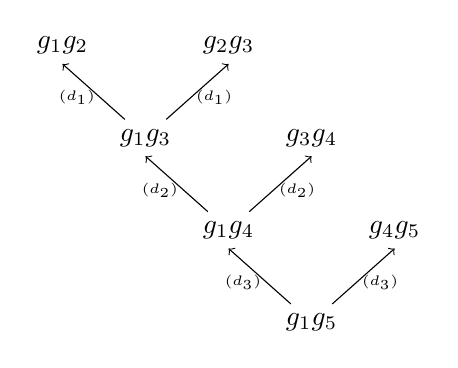
\begin{tikzpicture} [->, baseline=(current bounding box.center)]
    \node {$\subrulep{g_1}{g_5}$} [grow' = up, align=center, anchor=north,
                     sibling distance = 6em, level distance = 4em]
    child {node {$\subrulep{g_1}{g_4}$} 
      child {node {$\subrulep{g_1}{g_3}$}
        child {node {$\subrulep{g_1}{g_2}$}
                     edge from parent [child anchor=south]
                          node[below left=-0.4em] {$\scriptscriptstyle(d_1)$}
              }
        child {node {$\subrulep{g_2}{g_3}$}
                     edge from parent [child anchor=south]
                          node[below right=-0.4em] {$\scriptscriptstyle(d_1)$}
              }
                  edge from parent [child anchor=south]
                       node[below left=-0.4em] {$\scriptscriptstyle(d_2)$}
           }
      child {node {$\subrulep{g_3}{g_4}$}
                  edge from parent [child anchor=south]
                       node[below right=-0.4em] {$\scriptscriptstyle(d_2)$}}
              edge from parent [child anchor=south]
                  node[below left=-0.4em] {$\scriptscriptstyle(d_3)$}
            }
    child {node {$\subrulep{g_4}{g_5}$} edge from parent [child anchor=south]
                       node[below right=-0.4em] {$\scriptscriptstyle(d_3)$}
          };
    \end{tikzpicture}
    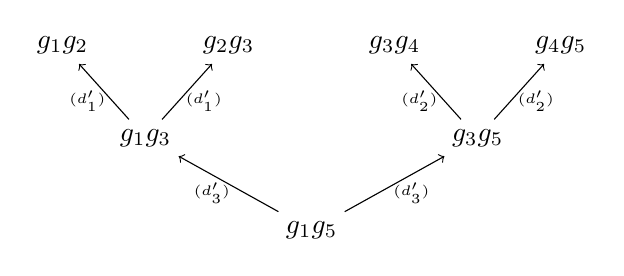
\begin{tikzpicture} [->, baseline=(current bounding box.center)]
    \node {$\subrulep{g_1}{g_5}$} [grow' = up, align=center, anchor=north,
                     sibling distance = 12em, level distance = 4em]
    child {node {$\subrulep{g_1}{g_3}$} [sibling distance=6em]
      child {node {$\subrulep{g_1}{g_2}$}
       edge from parent node[below left=-0.4em] {$\scriptscriptstyle(d_1')$}
            }
      child {node {$\subrulep{g_2}{g_3}$}
       edge from parent node[below right=-0.4em] {$\scriptscriptstyle(d_1')$}
            }
       edge from parent node[below left=-0.4em] {$\scriptscriptstyle(d_3')$}
          }
    child {node {$\subrulep{g_3}{g_5}$} [sibling distance=6em]
      child {node {$\subrulep{g_3}{g_4}$}
       edge from parent node[below left=-0.4em] {$\scriptscriptstyle(d_2')$}
            }
      child {node {$\subrulep{g_4}{g_5}$}
       edge from parent node[below right=-0.4em] {$\scriptscriptstyle(d_2')$}
            }
       edge from parent node[below right=-0.4em] {$\scriptscriptstyle(d_3')$}
          };
    \end{tikzpicture}
    \caption{Vertex-edge representations for \ref{def:ruleproofnot}-3 and
                                    \ref{def:ruleproofnot}-4}\label{fig:pt1}
     \end{figure}


  \def\transto#1{\hspace*{#1} &\rightsquigarrow \hspace*{#1}}
  \def\equivto#1{\hspace*{#1} &\equiv \hspace*{#1}}
  \def\sepval{0.5cm}
    \begin{align*}
    \tag{\ref{def:irulegraph}-1}
    \begin{prooftreem}
     \hypoi{\alpha_1~\alpha_2~\ldots~\alpha_{i-1}~\alpha_i~\alpha_{i+1}~
                      \ldots~\alpha_{k-1}~\alpha_k}
     \inferi{\beta}
    \end{prooftreem}
     \equivto{\sepval}
    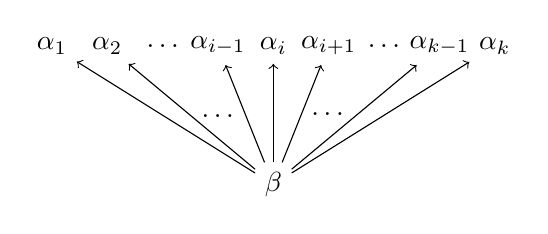
\begin{tikzpicture} [->, baseline=(current bounding box.center) ]
    \node {$\beta$} [grow' = up, align=center,
                     sibling distance = 2em, level distance = 5em]
    child {node {$\alpha_1$}}
    child {node {$\alpha_2$} edge from parent node [right] {$\ldots$}}
    child {node {$\ldots$} edge from parent [draw=none]}
    child {node {$\alpha_{i-1}$}}
    child {node {$\alpha_i$}}
    child {node {$\alpha_{i+1}$} edge from parent node [right] {$\ldots$}}
    child {node {$\ldots$} edge from parent [draw=none]}
    child {node {$\alpha_{k-1}$}}
    child {node {$\alpha_k$}};
    \end{tikzpicture}
    \\
    \tag{\ref{def:irulegraph}-2}
    \begin{prooftreem}
     \hypoi{\phantom{\true}}
     \inferi{\beta}
    \end{prooftreem}
     \equivto{\sepval}
    \begin{tikzpicture} [->, baseline=(current bounding box.center) ]
    \node {$\beta$} [grow = up, align=center,
                     sibling distance = 2em, level distance = 3em]
    child {node {$\true$}};
    \end{tikzpicture}
    \end{align*}


     child {node (tkm11) {$\treeupps{T_{(k\shortminus1)1}}$} \efpn}
     child {node (tkm12) {$\treeupps{T_{(k\shortminus1)2}}$} \efpn}
     child {\nodebldots{0.5} \efpn}
     child {node (tkm1jkm1m1) [xshift=-1em]
         {$\treeuppsb{T_{(k\shortminus1)({j_{k\shortminus1}\shortminus1)}}}$} \efpn}
     child {node (akm1jkm1) {$\mlnot\alpha_{(k\shortminus1)(j_{k\shortminus1})}$}
                                     edge from parent [<-]}
     child {node (tkm1jkm1p1) [xshift=1em]
                    {$\treeuppsb{T_{(k\shortminus1)({j_{k\shortminus1}}+1)}}$} \efpn}
     child {\nodebldots{0.5} \efpn}
     child {node (tkm1mkm1m1) [xshift=-1em]
            {$\treeuppsb{T_{(k\shortminus1)({m_{k\shortminus1}}\shortminus1)}}$} \efpn}
     child {node (tkm1mkm1) {$\treeuppsb{T_{(k\shortminus1)(m_{k\shortminus1})}}$}
            \efpn }


%%% T1x
    \draw (akm1jkm1.250) to[myncbar, arm=1.45,angle=270] (tkm11.south);
    \draw (akm1jkm1.235) to[myncbar, arm=1.35,angle=270] (tkm12.south);
    \draw (akm1jkm1.220) to[myncbar, arm=1.25,angle=270] (tkm1jkm1m1.south);
    \draw (akm1jkm1.320) to[myncbar, arm=1.25,angle=270] (tkm1jkm1p1.south);
    \draw (akm1jkm1.305) to[myncbar, arm=1.35,angle=270] (tkm1mkm1m1.south);
    \draw (akm1jkm1.290) to[myncbar, arm=1.45,angle=270] (tkm1mkm1.south);
%%% T2x
    \draw (akjk.250) to[myncbar, arm=1.45,angle=270] (tk1.south);
    \draw (akjk.235) to[myncbar, arm=1.35,angle=270] (tk2.south);
    \draw (akjk.220) to[myncbar, arm=1.25,angle=270] (tkjkm1.south);
    \draw (akjk.320) to[myncbar, arm=1.25,angle=270] (tkjkp1.south);
    \draw (akjk.305) to[myncbar, arm=1.35,angle=270] (tkmkm1.south);
    \draw (akjk.290) to[myncbar, arm=1.45,angle=270] (tkmk.south);
    \node (vdots1) [ above=1em of akm1jkm1] {$\vdots$};
    \draw [<-] (akm1jkm1) to (vdots1);
    \node (aip1jip1) [above=1em of vdots1]  {$\mlnot\alpha_{(i+1)(j_{i+1})}$}
                    [grow' = up, align=center, anchor=north,
                     sibling distance = 4em, level distance = 7em]
    child {node (ti1) {$\treeupps{T_{i1}}$}
                    edge from parent [child anchor=south, draw=none]}
    child {node (ti2) {$\treeupps{T_{i2}}$}
                    edge from parent [child anchor=south, draw=none]}
    child {\nodebldots{0.5} \efpn}
    child {node (tijim1) {$\treeupps{T_{i({j_i}\shortminus1)}}$}
                    edge from parent [child anchor=south, draw=none]}
    child {node (aiji) {$\mlnot\alpha_{i{j_i}}$} edge from parent [<-]}
    child {node (tijip1) {$\treeupps{T_{i({j_i}+1)}}$}
                    edge from parent [child anchor=south, draw=none]}
    child {\nodebldots{0.5} \efpn}
    child {node (timim1) {$\treeupps{T_{i({m_i}\shortminus1)}}$}
                    edge from parent [child anchor=south, draw=none]}
    child {node (timi) {$\treeupps{T_{i{m_i}}}$}
                    edge from parent [child anchor=south, draw=none]};
%%% Tix
    \draw (aiji.250) to[myncbar, arm=1.45,angle=270] (ti1.south);
    \draw (aiji.235) to[myncbar, arm=1.35,angle=270] (ti2.south);
    \draw (aiji.220) to[myncbar, arm=1.25,angle=270] (tijim1.south);
    \draw (aiji.320) to[myncbar, arm=1.25,angle=270] (tijip1.south);
    \draw (aiji.305) to[myncbar, arm=1.35,angle=270] (timim1.south);
    \draw (aiji.290) to[myncbar, arm=1.45,angle=270] (timi.south);
    \draw [<-] (vdots1) to (aip1jip1);
    \node (vdots2) [ above=1em of aiji] {$\vdots$};
    \draw [<-] (aiji) to (vdots2);
    \node (a3j3) [above=1em of vdots2] {$\mlnot\alpha_{3{j_3}}$}
                    [grow' = up, align=center, anchor=north,
                     sibling distance = 4em, level distance = 7em]
    child {node (t21) {$\treeupps{T_{21}}$}
                edge from parent [child anchor=south,draw=none]}
    child {node (t22) {$\treeupps{T_{22}}$}
                edge from parent [child anchor=south,draw=none]}
    child {\nodebldots{0.5} \efpn}
    child {node (t2j2m1) {$\treeupps{T_{2({j_2}\shortminus1)}}$}
                edge from parent [child anchor=south,draw=none]}
    child {node (a2j2) {$\mlnot\alpha_{2{j_2}}$} edge from parent [<-] 
     child {node (t11) {$\treeupps{T_{11}}$}
                edge from parent [child anchor=south,draw=none]}
     child {node (t12) {$\treeupps{T_{12}}$}
                edge from parent [child anchor=south,draw=none]}
     child {\nodebldots{0.5} \efpn}
     child {node (t1jm1) {$\treeupps{T_{1({j_1}\shortminus1)}}$}
                edge from parent [child anchor=south,draw=none]}
     child {node (a1j1) {$\mlnot\alpha_{1{j_1}}$} edge from parent [<-]}
     child {node (t1j1p1) {$\treeupps{T_{1({j_1}+1)}}$}
                edge from parent [child anchor=south,draw=none]}
     child {\nodebldots{0.5} \efpn}
     child {node (t1m1m1) {$\treeupps{T_{1({m_1}\shortminus1)}}$}
                edge from parent [child anchor=south,draw=none]}
     child {node (t1m1) {$\treeupps{T_{1m_1}}$}
                edge from parent [child anchor=south,draw=none]}
           }
    child {node (t2j2p1) {$\treeupps{T_{2({j_2}+1)}}$}
                edge from parent [child anchor=south,draw=none]}
    child {\nodebldots{0.5} \efpn}
    child {node (t2m2m1) {$\treeupps{T_{2({m_2}\shortminus1)}}$}
                edge from parent [child anchor=south,draw=none]}
    child {node (t2m2) {$\treeupps{T_{2{m_2}}}$}
               edge from parent [child anchor=south,draw=none]};
    \draw [<-] (vdots2) to (a3j3);
%%% T1x
    \draw (a1j1.250) to[myncbar, arm=1.45,angle=270] (t11.south);
    \draw (a1j1.235) to[myncbar, arm=1.35,angle=270] (t12.south);
    \draw (a1j1.220) to[myncbar, arm=1.25,angle=270] (t1jm1.south);
    \draw (a1j1.290) to[myncbar, arm=1.45,angle=270] (t1m1.south);
    \draw (a1j1.305) to[myncbar, arm=1.35,angle=270] (t1m1m1.south);
    \draw (a1j1.320) to[myncbar, arm=1.25,angle=270] (t1j1p1.south);
%%% T2x
    \draw (a2j2.250) to[myncbar, arm=1.45,angle=270] (t21.south);
    \draw (a2j2.235) to[myncbar, arm=1.35,angle=270] (t22.south);
    \draw (a2j2.220) to[myncbar, arm=1.25,angle=270] (t2j2m1.south);
    \draw (a2j2.320) to[myncbar, arm=1.25,angle=270] (t2j2p1.south);
    \draw (a2j2.305) to[myncbar, arm=1.35,angle=270] (t2m2m1.south);
    \draw (a2j2.290) to[myncbar, arm=1.45,angle=270] (t2m2.south);


      \def\markneg#1{#1}
     \def\hsepc{\hspace*{1em}}
%     \def\hsepc{\relax}
     \begin{figure}[htb]
    \begin{tikzpicture} [->, baseline=(current bounding box.center) ]
    \node (beta) {$\mlnot\beta$} [grow' = up, align=center, anchor=north,
                     sibling distance = 4em, level distance = 7em]
    child {node (tk1) {$\treeupps{T_{k1}}$} \efpn}
    child {node (tk2) {$\treeupps{T_{k2}}$} \efpn}
    child {\nodebldots{0.5} \efpn}
    child {node (tkjkm1) {$\treeupps{T_{k({j_k}\shortminus1)}}$} \efpn}
    child {node (akjk) {$\mlnot\alpha_{k{j_k}}$} edge from parent [<-]
          }
    child {node (tkjkp1) {$\treeupps{T_{k({j_k}+1)}}$}
                    edge from parent [child anchor=south, draw=none]}
    child {\nodebldots{0.5} \efpn}
    child {node (tkmkm1) {$\treeupps{T_{k({m_k}\shortminus1)}}$}
                    edge from parent [child anchor=south, draw=none]}
    child {node (tkmk) {$\treeupps{T_{k{m_k}}}$}
                    edge from parent [child anchor=south, draw=none]};



%    \draw (vdots2) to (a3j3);
    \end{tikzpicture}
     \caption{The contrapositioned proof II}\label{fig:contrapii}
     \end{figure}




      \def\markneg#1{#1}
     \def\hsepc{\hspace*{1em}}
%     \def\hsepc{\relax}
     \begin{figure}[htb]
    \begin{tikzpicture} [->, baseline=(current bounding box.center) ]
    \node {$\mlnot\alpha_{1{j_1}}$} [grow' = up, align=center, anchor=north,
                     sibling distance = 4em, level distance = 7em]
    child {node {$\treeupps{T_{11}}$} \efpas}
    child {node {$\treeupps{T_{12}}$} \efpas \noderldots{1.75} }
    child {node [below=2em] {$\ldots$} \efpn}
    child {node {$\treeupps{T_{1({j_1}\shortminus1)}}$} \efpas}
    child {node {$\mlnot\alpha_{2{j_2}}$}
     child {node {$\treeupps{T_{21}}$} \efpas}
     child {node {$\treeupps{T_{22}}$}  \efpas \noderldots{1.75} }
     child {node [below=2em] {$\ldots$} \efpn}
     child {node %[xshift=-1em]
                    {$\treeupps{T_{2(j_2\shortminus1)}}$}
                                     \efpas}
     child {node (akm1jkm1) {$\mlnot\alpha_{3j_3}$}}
     child {node %[xshift=1em]
                    {$\treeupps{T_{2({j_2}+1)}}$}
                                     \efpas
                                     node [right=1.75em] {$\ldots$}} 
     child {node [below=2em] {$\ldots$} \efpn}
     child {node {$\treeupps{T_{2({m_2}\shortminus1)}}$} \efpas
           }
     child {node {$\treeupps{T_{2m_2}}$} \efpas
           }
    child {node {$\treeupps{T_{1({j_1}+1)}}$} \efpas
                                     node [right=1.75em] {$\ldots$}
          }
    child {node [below=2em] {$\ldots$} \efpn}
    child {node {$\treeupps{T_{1({m_1}\shortminus1)}}$} \efpas}
    child {node {$\treeupps{T_{1{m_1}}}$} \efpas};
    \node (vdots1) [ above=1em of akm1jkm1] {$\vdots$};
    \draw (akm1jkm1) to (vdots1);
    \node (aip1jip1) [above=1em of vdots1]  {$\mlnot\alpha_{i{j_i}}$}
                    [grow' = up, align=center, anchor=north,
                     sibling distance = 4em, level distance = 7em]
    child {node {$\treeupps{T_{i1}}$} \efpas}
    child {node {$\treeupps{T_{i2}}$} \efpas
                                     node [right=1.75em] {$\ldots$}}
    child {node [below=2em] {$\ldots$} \efpn}
    child {node [xshift=-1em] {$\treeupps{T_{i({j_i}\shortminus1)}}$}
                                     \efpas}
    child {node (aiji) {$\mlnot\alpha_{(i+1){j_{i+1}}}$}}
    child {node [xshift=1em] {$\treeupps{T_{i({j_i}+1)}}$}
                                     \efpas
                                     node [right=1.75em] {$\ldots$}}
    child {node [below=2em] {$\ldots$} \efpn}
    child {node {$\treeupps{T_{i({m_i}\shortminus1)}}$}
                                     \efpas}
    child {node {$\treeupps{T_{i{m_i}}}$}
                                     \efpas};
    \draw (vdots1) to (aip1jip1);
    \node (vdots2) [ above=1em of aiji] {$\vdots$};
    \draw (aiji) to (vdots2);
    \node (a3j3) [above=1em of vdots2]
                     {$\mlnot\alpha_{(k\shortminus1){j_{(k\shortminus1)}}}$}
                    [grow' = up, align=center, anchor=north,
                     sibling distance = 4em, level distance = 7em]
    child {node {$\treeupps{T_{(k\shortminus1)1}}$}
                     \efpas}
    child {node {$\treeupps{T_{(k\shortminus1)2}}$}
                     \efpas
                                     node [right=1.75em] {$\ldots$}}
    child {node [below=2em] {$\ldots$} \efpn}
    child {node {$\treeuppsb{T_{(k\shortminus1)({j_{k\shortminus1}}\shortminus1)}}$}
                                     \efpas}
    child {node (a2i2) {$\mlnot\alpha_{k{j_k}}$}
     child {node {$\treeupps{T_{k1}}$}
                                      \efpas}
     child {node {$\treeupps{T_{k2}}$} \efpas
                                      node [right=1.75em] {$\ldots$}}
     child {node [below=2em] {$\ldots$} \efpn}
     child {node {$\treeupps{T_{k({j_k}\shortminus1)}}$}
                                     \efpas}
     child {node (a1i1) {$\mlnot\beta$}}
     child {node {$\treeupps{T_{k({j_k}+1)}}$}
                                     \efpas
                                     node [right=1.75em] {$\ldots$}} 
     child {node [below=2em] {$\ldots$} \efpn}
     child {node {$\treeupps{T_{k({m_k}\shortminus1)}}$}
                                     \efpas}
     child {node {$\treeupps{T_{1m_k}}$}
                                     \efpas}
           }
    child {node {$\treeuppsb{T_{(k\shortminus1)({j_{k\shortminus1}}+1)}}$}
                                     \efpas
                                     node [right=1.75em] {$\ldots$}}
    child {node [below=2em] {$\ldots$} \efpn}
    child {node [xshift=-1em]
                 {$\treeuppsb{T_{(k\shortminus1)({m_{k\shortminus1}}\shortminus1)}}$}
                                     \efpas}
    child {node {$\treeuppsb{T_{(k\shortminus1){m_{k\shortminus1}}}}$}
                                     \efpas};
    \end{tikzpicture}
     \caption{The contrapositioned proof I}\label{fig:contrapi}
     \end{figure}

 \begin{metalabpara}{discussion}{}
     {Total completeness in the Armstrong
                             setting}\envlabel{disc:totalarmcompl}
    It is possible to augment
 \preformat{\linebreak}
 $\swapcl{\proofsys{A}}$ to render it
totally complete, even for deducing unsatisfiability.  The idea is as
follows.  For each rule of the form
     \[
       \tag{\ref{disc:totalarmcompl}-1}
       \begin{prooftree}
         \hypoi{\alpha_1~\alpha_2~\ldots~\alpha_k}
         \inferi{\beta}
       \end{prooftree}
     \]
 add one of the form
     \[
       \tag{\ref{disc:totalarmcompl}-2}
       \begin{prooftree}
         \hypoi{\alpha_1~\alpha_2~\ldots~\alpha_k~~\mlnot\beta}
         \inferi{\false}
       \end{prooftree}
     \]
  In (\ref{disc:totalarmcompl}-1), all formulas are in
  $\allarm{\armctxt{C}}$; that is, they may be positive or negative.
    \par
   This should work for any deductive system whose formulas are closed
under complement..
    \par
   This topic is not pursued further here because it is not central to
the problem at hand.
 \end{metalabpara}


 \begin{metalabpara}{myexample}{Example}
    {Inference involving negative assertions}\envlabel{ex:neg}
   Let
  \nlrightt
   $\Phi = \setbr{\subrulep[\gsn]{g_1}{g_2},
                      \subrulep[\gsn]{g_2}{g_3},
                      \subrulep[\gsn]{g_4}{g_5},
                      \subrulep[\gsn]{g_5}{g_6},
                      \nsubrulep[\gsn]{g_1}{g_6}}$.
   \linebreak
   It is not difficult to see that 
     $\Phi \sentailsd{\gsn} \nsubrulep[\gsn]{g_3}{g_4}$
 and that $\Phi$ is minimal in that regard.
   Indeed, that statement holds iff
  \nlrightt
  $\posof{\Phi} \union \subrulep[\gsn]{g_3}{g_4}
             \sentailsd{\gsn} \subrulep[\gsn]{g_1}{g_6}$,
 \linebreak
 as a simple application of \envref{lem:genswap} shows.
   \newline
   To show that the latter entailment holds, begin by expanding
$\posof{\Phi}$, obtaining
     \nlrightt
   $\subrulep[\gsn]{g_1}{g_2},
                      \subrulep[\gsn]{g_2}{g_3},
                      \subrulep[\gsn]{g_4}{g_5},
                      \subrulep[\gsn]{g_5}{g_6}
             \sentailsd{\gsn} \subrulep[\gsn]{g_1}{g_6}$.
 \newline
   Shown in (\ref{ex:neg}-1) is the corresponding proof tree,
corresponding to that of Fig.\ \ref{fig:toflip}, which will undergo
undergo the swap process, with the statements to be involved in the
swap marked with an asterisk.
   \begin{figure}[htb]
  \def\swapsquigarrow{\shortstack{\mbox{\footnotesize swap}\\ \rightsquigarrow}}
  \def\transto#1{\hspace*{#1} \swapsquigarrow \hspace*{#1}}
  \def\equivto#1{\hspace*{#1} \equiv \hspace*{#1}}
  \def\sepval{0.5cm}
    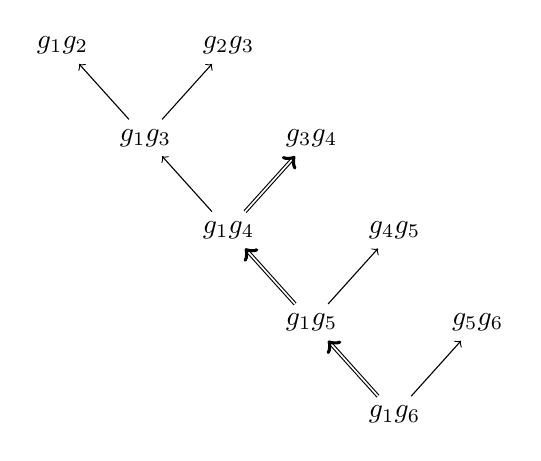
\begin{tikzpicture} [->, baseline=(current bounding box.center)]
    \node {$\subrulep{g_1}{g_6}$} [grow' = up, align=center, anchor=north,
                     sibling distance = 6em, level distance = 4em]
    child {node {$\subrulep{g_1}{g_5}$} edge from parent [double]
      child {node {$\subrulep{g_1}{g_4}$} edge from parent [double]
        child {node {$\subrulep{g_1}{g_3}$}
          child {node {$\subrulep{g_1}{g_2}$}}
          child {node {$\subrulep{g_2}{g_3}$}}
              }
        child {node {$\subrulep{g_3}{g_4}$} edge from parent [double]
              }
            }
      child {node {$\subrulep{g_4}{g_5}$}
            }
          }
    child {node {$\subrulep{g_5}{g_6}$}};
    \end{tikzpicture}
    \hspace*{-2em}\smash{\transto{0em}}\hspace{-2em}
    \begin{tikzpicture} [->, %every edge/.style={draw=none},
                         baseline=(current bounding box.center)]
    \node (g16) {$\nsubrulep{g_1}{g_6}$}
                    [grow' = up, align=center, anchor=north,
                     sibling distance = 6em, level distance = 4em]
    child {node (g15) {$\nsubrulep{g_1}{g_5}$} \efpn
      child {node (g14) {$\nsubrulep{g_1}{g_4}$} \efpn
        child {node (g13) {$\subrulep{g_1}{g_3}$} \efpn
          child {node (g12) {$\subrulep{g_1}{g_2}$}}
          child {node (g11) {$\subrulep{g_2}{g_3}$}}
              }
        child {node (g34) {$\nsubrulep{g_3}{g_4}$} \efpn}
            } 
      child {node (g45) {$\subrulep{g_4}{g_5}$} \efpn}
          }
    child {node (g56) {$\subrulep{g_5}{g_6}$} \efpn};
    \draw (g15) edge [double,->] (g16);
    \draw (g15) edge [dashed,->] (g56);
    \draw (g14) edge [double,->] (g15);
    \draw (g14) edge [dashed,->] (g45);
    \draw (g34) edge [double,->] (g14);
    \draw (g34) edge [dashed,->] (g13);
    \end{tikzpicture}
    \\[1em]
    \phantom{xxxxx}\hfill\equivto{\sepval}
    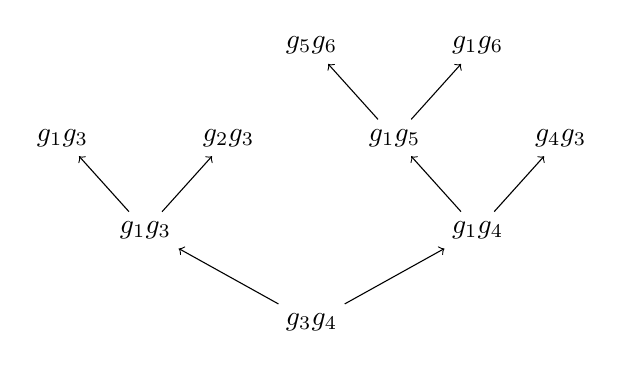
\begin{tikzpicture} [->, baseline=(current bounding box.center),
           level 1/.style={sibling distance=12em},
           level 2/.style={sibling distance=6em},
           level 3/.style={sibling distance=6em}
                        ]
    \node {$\nsubrulep{g_3}{g_4}$} [grow' = up, align=center, anchor=north,
                     level distance = 4em]
    child {node {$\subrulep{g_1}{g_3}$}
      child {node {$\subrulep{g_1}{g_3}$}}
      child {node {$\subrulep{g_2}{g_3}$}}
          }
    child {node {$\nsubrulep{g_1}{g_4}$}
      child {node {$\nsubrulep{g_1}{g_5}$}
        child {node {$\subrulep{g_5}{g_6}$}}
        child {node {$\nsubrulep{g_1}{g_6}$}}
            }
      child {node {$\subrulep{g_4}{g_3}$}}
          };
    \end{tikzpicture}
    \caption{Example1}\label{fig:example1}
    \end{figure}
 \[
    \tag{\ref{ex:neg}-1}
    \begin{prooftreem}
     \hypoii{\subrulep[\gsn]{g_1}{g_2}}
            {\subrulep[\gsn]{g_2}{g_3}}
     \inferi{\subrulep[\gsn]{g_1}{g_3}}
     \hypoi{\markneg{\subrulep[\gsn]{g_3}{g_4}}}
     \inferii{\markneg{\subrulep[\gsn]{g_1}{g_4}}}
     \hypoi{\subrulep[\gsn]{g_4}{g_5}}
     \inferii{\markneg{\subrulep[\gsn]{g_1}{g_5}}}
     \hypoi{\subrulep[\gsn]{g_5}{g_6}}
     \inferii{\markneg{\subrulep[\gsn]{g_1}{g_6}}}
    \end{prooftreem}
 \]
    The individual swaps to be executed are shown in (\ref{ex:neg}-2),
again with the elements to be swapped tagged with an asterisk.

 \begin{align*}
    \tag{\ref{ex:neg}-2}
    \begin{prooftreem}
     \hypoii{\markneg{\subrulep[\gsn]{g_1}{g_5}}}
            {\subrulep[\gsn]{g_5}{g_6}}
     \inferi{\markneg{\subrulep[\gsn]{g_1}{g_6}}}
    \end{prooftreem}
    \quad &\rightsquigarrow \quad
    \begin{prooftreem}
     \hypoii{\subrulep[\gsn]{g_5}{g_6}}
            {\nsubrulep[\gsn]{g_1}{g_6}}
     \inferi{\nsubrulep[\gsn]{g_1}{g_5}}
    \end{prooftreem} \\
    \begin{prooftreem}
     \hypoii{\markneg{\subrulep[\gsn]{g_1}{g_4}}}
            {\subrulep[\gsn]{g_4}{g_5}}
     \inferi{\markneg{\subrulep[\gsn]{g_1}{g_5}}}
    \end{prooftreem}
    \quad &\rightsquigarrow \quad
    \begin{prooftreem}
     \hypoii{\subrulep[\gsn]{g_4}{g_5}}
            {\nsubrulep[\gsn]{g_1}{g_5}}
     \inferi{\nsubrulep[\gsn]{g_1}{g_4}}
    \end{prooftreem} \\
    \begin{prooftreem}
     \hypoii{\markneg{\subrulep[\gsn]{g_1}{g_3}}}
            {\subrulep[\gsn]{g_3}{g_4}}
     \inferi{\markneg{\subrulep[\gsn]{g_1}{g_4}}}
    \end{prooftreem}
    \quad &\rightsquigarrow \quad
    \begin{prooftreem}
     \hypoii{\subrulep[\gsn]{g_1}{g_3}}
            {\nsubrulep[\gsn]{g_1}{g_4}}
     \inferi{\nsubrulep[\gsn]{g_3}{g_4}}
    \end{prooftreem}
 \end{align*}
   Finally, (\ref{ex:neg}-3) shows the final, desired proof tree,
after the swaps have been executed, corresponding to the general case
of Fig.\ \ref{fig:flipped}.
 \[
    \tag{\ref{ex:neg}-3}
    \begin{prooftreem}
     \hypoii{\subrulep[\gsn]{g_1}{g_2}}
            {\subrulep[\gsn]{g_2}{g_3}}
     \inferi{\subrulep[\gsn]{g_1}{g_3}}
     \hypoii{\subrulep[\gsn]{g_5}{g_6}}
            {\nsubrulep[\gsn]{g_1}{g_6}}
     \inferi{\nsubrulep[\gsn]{g_1}{g_5}}
     \hypoi{\subrulep[\gsn]{g_4}{g_5}}
     \inferii{\nsubrulep[\gsn]{g_1}{g_4}}
     \inferii{\nsubrulep[\gsn]{g_3}{g_4}}
    \end{prooftreem}
 \]

 \end{metalabpara}


 \begin{metalabpara}{myexample}{Example}
    {Inference involving negative assertions 2}\envlabel{ex:negii}
   In this example, a proof of a negated assertion from an
all-positive set of antecedents will be elaborated.
   Let
   \nlrightt
   $\Phi =
   \setbr{\subrulep[\gsn]{g_1}{g_2},
          \subrulep[\gsn]{g_2}{g_4},
          \subrulep[\gsn]{g_4}{g_6},
          \subrulep[\gsn]{g_3}{g_5},
          \subrulep[\gsn]{g_5}{g_7},
          \disjrulep[\gsn]{g_6}{g_7}}$.
   \linebreak
   To prove
   $\Phi \sentails \nsubrulep[\gsn]{g_1}{g_3}$,
   it suffices to prove that
   $\Phi \union \setbr{\subrulep[\gsn]{g_1}{g_3}} \sentails \false$.
   Shown in (\ref{ex:neg}-1) is the proof tree corresponding to
Fig.\ \ref{fig:toflip}, again with the items to be swapped marked with
an asterisk.

 {\footnotesize
 \[
    \tag{\ref{ex:neg}-1}
    \begin{prooftreem}
     \hypoii{\subrulep[\gsn]{g_1}{g_2}}
            {\subrulep[\gsn]{g_2}{g_4}}
     \inferi{\subrulep[\gsn]{g_1}{g_4}}
     \hypoi{\subrulep[\gsn]{g_4}{g_6}}
     \inferii{\subrulep[\gsn]{g_1}{g_6}}
     \hypoii{\markneg{\subrulep[\gsn]{g_1}{g_3}}}
            {\subrulep[\gsn]{g_3}{g_5}}
     \inferi{\markneg{\subrulep[\gsn]{g_1}{g_5}}}
     \hypoi{\subrulep[\gsn]{g_5}{g_7}}
     \inferii{\markneg{\subrulep[\gsn]{g_1}{g_7}}}
     \hypoi{\disjrulep{g_6}{g_7}}
     \inferiii{\markneg{\disjrulesetp{\setbr{g_1}}}}
     \inferi{\markneg{\false}}
    \end{prooftreem}
 \]
 }
 \noindent
   Shown in (\ref{ex:neg}-2) are the individual swaps which must be
applied to establish that $\Phi \sentailsd{\gsn}
\nsubrulep[\gsn]{g_3}{g_4}$:
 \begin{align*}
    \tag{\ref{ex:neg}-2}
    \begin{prooftreem}
     \hypoii{\markneg{\subrulep[\gsn]{g_1}{g_3}}}
            {\subrulep[\gsn]{g_3}{g_5}}
     \inferi{\markneg{\subrulep[\gsn]{g_1}{g_5}}}
    \end{prooftreem}
    \quad &\rightsquigarrow \quad
    \begin{prooftreem}
     \hypoii{\nsubrulep[\gsn]{g_1}{g_5}}
            {\subrulep[\gsn]{g_3}{g_5}}
     \inferi{\nsubrulep[\gsn]{g_1}{g_3}}
    \end{prooftreem} \\
    \begin{prooftreem}
     \hypoii{\markneg{\subrulep[\gsn]{g_3}{g_5}}}
            {\subrulep[\gsn]{g_5}{g_7}}
     \inferi{\markneg{\subrulep[\gsn]{g_3}{g_7}}}
    \end{prooftreem}
    \quad &\rightsquigarrow \quad
    \begin{prooftreem}
     \hypoii{\nsubrulep[\gsn]{g_3}{g_7}}
            {\subrulep[\gsn]{g_5}{g_7}}
     \inferi{\nsubrulep[\gsn]{g_3}{g_5}}
    \end{prooftreem} \\
    \begin{prooftreem}
     \hypoiii{\subrulep[\gsn]{g_1}{g_6}}
             {\markneg{\subrulep[\gsn]{g_1}{g_7}}}
             {\markneg{\disjrulep{g_6}{g_7}}}
     \inferi{\markneg{\disjrulesetp{\setbr{g_1}}}}
    \end{prooftreem}
    \quad &\rightsquigarrow \quad
    \begin{prooftreem}
     \hypoiii{\subrulep[\gsn]{g_1}{g_6}}
            {\disjrulep[\gsn]{g_6}{g_7}}
            {\ndisjrulesetp[\gsn]{\setbr{g_1}}}
     \inferi{\nsubrulep[\gsn]{g_1}{g_7}}
    \end{prooftreem} \\
    \begin{prooftreem}
     \hypoi{\markneg{\disjrulesetp{\setbr{g_1}}}}
           {\false}
     \inferi{\markneg{\nsubrulep[\gsn]{g_1}{g_7}}}
    \end{prooftreem}
    \quad &\rightsquigarrow \quad
    \begin{prooftreem}
     \hypoi{}
     \inferi{\ndisjrulesetp{\setbr{g_1}}}
    \end{prooftreem} \\
 \end{align*}

  Finally, shown in (\ref{ex:neg}-3) is the application of these
swaps, according to the transition from
 Fig.\ \ref{fig:toflip} to Fig.\ \ref{fig:flipped}.

 \[
    \tag{\ref{ex:neg}-3}
    \footnotesize
    \begin{prooftreem}
     \hypoii{\subrulep[\gsn]{g_1}{g_2}}
            {\subrulep[\gsn]{g_2}{g_4}}
     \inferi{\subrulep[\gsn]{g_1}{g_4}}
     \hypoi{\subrulep[\gsn]{g_4}{g_6}}
     \inferii{\subrulep[\gsn]{g_1}{g_6}}
     \hypoi{}
     \inferi{\ndisjrulesetp[\gsn]{\setbr{g_1}}}
     \hypoi{\disjrulep[\gsn]{g_6}{g_7}}
     \inferiii{\nsubrulep[\gsn]{g_1}{g_7}}
     \hypoi{\subrulep[\gsn]{g_5}{g_7}}
     \inferii{\nsubrulep[\gsn]{g_1}{g_5}}
     \hypoi{\subrulep{g_3}{g_5}}
     \inferii{\nsubrulep[\gsn]{g_1}{g_3}}
    \end{prooftreem}
 \]

   \begin{figure}[htbp]
    \begin{tikzpicture} [->, baseline=(current bounding box.center),
           level 1/.style={sibling distance=6em},
           level 2/.style={sibling distance=12em},
           level 3/.style={sibling distance=6em}
                        ]
    \node {$\false$} [grow' = up, align=center, anchor=north,
                      level distance = 4em]
      child {node {$\disjrulesetp{\setbr{g_1}}$} edge from parent [double]
        child {node {$\subrulep{g_1}{g_6}$} 
          child {node {$\subrulep{g_1}{g_4}$}
            child {node {$\subrulep{g_1}{g_2}$}}
            child {node {$\subrulep{g_2}{g_4}$}}
                }
          child {node {$\subrulep{g_4}{g_6}$}}
              }
        child {node {$\subrulep{g_1}{g_7}$} edge from parent [double]
          child {node {$\subrulep{g_1}{g_5}$} edge from parent [double]
            child {node {$\subrulep{g_1}{g_3}$} edge from parent [double]}
            child {node {$\subrulep{g_3}{g_5}$}}
                }
          child {node {$\subrulep{g_5}{g_7}$}}
              }
        child {node {$\disjrulep{g_6}{g_7}$}}
            };
    \end{tikzpicture}
    \begin{tikzpicture} [->, %every edge/.style={draw=none},
                         baseline=(current bounding box.center),
           level 1/.style={sibling distance=6em},
           level 2/.style={sibling distance=12em},
           level 3/.style={sibling distance=6em}
                        ]
    \node (f) {$\true$} [grow' = up, align=center, anchor=north,
                     sibling distance = 6em, level distance = 4em]
      child {node (g1) {$\ndisjrulesetp{\setbr{g_1}}$}
                       \efpn
        child {node (g16) {$\subrulep{g_1}{g_6}$}
                            \efpn
          child {node (g14) {$\subrulep{g_1}{g_4}$}
            child {node (g12) {$\subrulep{g_1}{g_2}$}}
            child {node (g24) {$\subrulep{g_2}{g_4}$}}
               }
          child {node (g46) {$\subrulep{g_4}{g_6}$}}
              }
        child {node (g17) {$\nsubrulep{g_1}{g_7}$}
                            \efpn
          child {node (g15) {$\nsubrulep{g_1}{g_5}$}
                             \efpn
            child {node (g13) {$\nsubrulep{g_1}{g_3}$}
                               \efpn}
            child {node (g35) {$\subrulep{g_3}{g_5}$}
                               \efpn}
                }
          child {node (g57) {$\subrulep{g_5}{g_7}$}
                             \efpn}
              }
        child {node (g67) {$\disjrulep{g_6}{g_7}$}
                            \efpn}
            };
    \draw (g1) edge [->,double]  (f) ;
    \draw (g17) edge [->,double] (g1);
    \draw (g17) edge [->,dashed] (g16);
    \draw (g17) edge [->,dashed] (g67);
    \draw (g15) edge [->,double] (g17);
    \draw (g15) edge [->,dashed] (g57);
    \draw (g13) edge [->,dashed] (g35);
    \draw (g13) edge [->,double] (g15);
    \end{tikzpicture}
    \begin{tikzpicture} [->, baseline=(current bounding box.center),
           level 1/.style={sibling distance=6em},
           level 2/.style={sibling distance=6em},
           level 3/.style={sibling distance=8em},
           level 4/.style={sibling distance=6em}
                        ]
    \node {$\nsubrulep{g_1}{g_3}$} [grow' = up, align=center, anchor=north,
                     level distance = 4em]
    child {node {$\nsubrulep{g_1}{g_5}$}   
      child {node {$\nsubrulep{g_1}{g_7}$}
        child {node {$\subrulep{g_1}{g_6}$}
          child {node {$\subrulep{g_1}{g_4}$}
            child {node {$\subrulep{g_1}{g_3}$}}
            child {node {$\subrulep{g_3}{g_4}$}}
                }
          child {node {$\subrulep{g_4}{g_6}$}}
              }
        child {node {$\ndisjrulesetp{\setbr{g_1}}$}
          child {node {$\true$}}
              }
        child {node {$\disjrulep{g_6}{g_7}$}}
            }
      child {node {$\subrulep{g_5}{g_7}$}}
          }
    child {node {$\nsubrulep{g_3}{g_5}$}
          };
    \end{tikzpicture}
    \caption{Example2}\label{fig:example2}
    \end{figure}

 \end{metalabpara}


 \begin{metalabpara}{myexample}{Example}
    {Inference involving negative assertions 2}\envlabel{ex:neginf2}
   In this example, a proof of a negated assertion from an
all-positive set of antecedents is examined.
   Let
   \nlrightt
   $\Phi =
   \setbr{\subrulep[\gsn]{g_1}{g_2},
          \subrulep[\gsn]{g_2}{g_4},
          \subrulep[\gsn]{g_4}{g_6},
          \subrulep[\gsn]{g_3}{g_5},
          \subrulep[\gsn]{g_5}{g_7},
          \disjrulep[\gsn]{g_6}{g_7}}$.
   \linebreak
   To prove
   $\Phi \sentails \nsubrulep[\gsn]{g_1}{g_3}$,
   it suffices to show that
   $\Phi \union \setbr{\subrulep[\gsn]{g_1}{g_3}} \sentails \false$.
   \begin{figure}[htbp]
  \def\swapsquigarrow{\shortstack{\mbox{\footnotesize swap}\\ \rightsquigarrow}}
  \def\transto#1{\hspace*{#1} \swapsquigarrow \hspace*{#1}}
  \def\equivto#1{\hspace*{#1} \equiv \hspace*{#1}}
  \def\sepval{0.5cm}
    \begin{tikzpicture} [->, baseline=(current bounding box.center),
           level 1/.style={sibling distance=6em},
           level 2/.style={sibling distance=12em},
           level 3/.style={sibling distance=6em}
                        ]
    \node {$\false$} [grow' = up, align=center, anchor=north,
                      level distance = 4em]
      child {node {$\disjrulesetp{\setbr{g_1}}$} edge from parent [double]
        child {node {$\subrulep{g_1}{g_6}$} 
          child {node {$\subrulep{g_1}{g_4}$}
            child {node {$\subrulep{g_1}{g_2}$}}
            child {node {$\subrulep{g_2}{g_4}$}}
                }
          child {node {$\subrulep{g_4}{g_6}$}}
              }
        child {node {$\subrulep{g_1}{g_7}$} edge from parent [double]
          child {node {$\subrulep{g_1}{g_5}$} edge from parent [double]
            child {node {$\subrulep{g_1}{g_3}$} edge from parent [double]}
            child {node {$\subrulep{g_3}{g_5}$}}
                }
          child {node {$\subrulep{g_5}{g_7}$}}
              }
        child {node {$\disjrulep{g_6}{g_7}$}}
            };
    \end{tikzpicture}
    \\[1em]
    \phantom{xxxxx}\transto{-0.6em}
    \begin{tikzpicture} [->, %every edge/.style={draw=none},
                         baseline=(current bounding box.center),
           level 1/.style={sibling distance=6em},
           level 2/.style={sibling distance=12em},
           level 3/.style={sibling distance=6em}
                        ]
    \node (f) {$\true$} [grow' = up, align=center, anchor=north,
                     sibling distance = 6em, level distance = 4em]
      child {node (g1) {$\ndisjrulesetp{\setbr{g_1}}$}
                       \efpn
        child {node (g16) {$\subrulep{g_1}{g_6}$}
                            \efpn
          child {node (g14) {$\subrulep{g_1}{g_4}$}
            child {node (g12) {$\subrulep{g_1}{g_2}$}}
            child {node (g24) {$\subrulep{g_2}{g_4}$}}
               }
          child {node (g46) {$\subrulep{g_4}{g_6}$}}
              }
        child {node (g17) {$\nsubrulep{g_1}{g_7}$}
                            \efpn
          child {node (g15) {$\nsubrulep{g_1}{g_5}$}
                             \efpn
            child {node (g13) {$\nsubrulep{g_1}{g_3}$}
                               \efpn}
            child {node (g35) {$\subrulep{g_3}{g_5}$}
                               \efpn}
                }
          child {node (g57) {$\subrulep{g_5}{g_7}$}
                             \efpn}
              }
        child {node (g67) {$\disjrulep{g_6}{g_7}$}
                            \efpn}
            };
    \draw (g1) edge [->,double]  (f) ;
    \draw (g17) edge [->,double] (g1);
    \draw (g17) edge [->,dashed] (g16);
    \draw (g17) edge [->,dashed] (g67);
    \draw (g15) edge [->,double] (g17);
    \draw (g15) edge [->,dashed] (g57);
    \draw (g13) edge [->,dashed] (g35);
    \draw (g13) edge [->,double] (g15);
    \end{tikzpicture}
    \\[1em]
    \phantom{xxxxx}\equivto{0em}\hfill
    \begin{tikzpicture} [->, baseline=(current bounding box.center),
           level 1/.style={sibling distance=6em},
           level 2/.style={sibling distance=6em},
           level 3/.style={sibling distance=8em},
           level 4/.style={sibling distance=6em}
                        ]
    \node {$\nsubrulep{g_1}{g_3}$} [grow' = up, align=center, anchor=north,
                     level distance = 4em]
    child {node {$\nsubrulep{g_1}{g_5}$}   
      child {node {$\nsubrulep{g_1}{g_7}$}
        child {node {$\subrulep{g_1}{g_6}$}
          child {node {$\subrulep{g_1}{g_4}$}
            child {node {$\subrulep{g_1}{g_3}$}}
            child {node {$\subrulep{g_3}{g_4}$}}
                }
          child {node {$\subrulep{g_4}{g_6}$}}
              }
        child {node {$\ndisjrulesetp{\setbr{g_1}}$}
          child {node {$\true$}
          edge from parent [double]
                }
          edge from parent [double]
              }
        child {node {$\disjrulep{g_6}{g_7}$}}
          edge from parent [double]
            }
      child {node {$\subrulep{g_5}{g_7}$}}
          edge from parent [double]
          }
    child {node {$\nsubrulep{g_3}{g_5}$}
          };
    \end{tikzpicture}
    \caption{Proof trees for \envref{ex:neginf2}}\label{fig:neginf2}
    \end{figure}
   In a similar manner to that used in Fig.\ \ref{fig:neginf1} for
\envref{ex:neginf1}, Fig.\ \ref{fig:neginf2} shows the sequence of
three trees, the concrete instantiations of
Figs.\ \ref{fig:tocontrap}, \ref{fig:contrapi}, and
\ref{fig:contrapii} for this example.  As in \envref{ex:neginf1}, the
double-line arrows identify the swap path, while the dashed lines in
the second tree identify those edges whose source vertex was changed
by the swap.
 \end{metalabpara}


 \begin{metalabpara}{mydefinition}{}
         {The doublet subsumption graph of an SMAS}\envlabel{def:sgraphii}
    In a disjointness rule of the form $\disjrulep{g_1}{g_2}$, the
argument is in most cases an unordered pair of distinct\footnote{
    The case in which the granules are not distinct, \ie, when
 $g_1 \ideq g_2$, is covered in \envref{def:effunary}.
                  }
 granules, called a doublet.
    Formally, the set of \emph{doublets} of $\granschemaname{G}$ is
defined to be
   $\doubletsofgrsch{G} =
      \setdef{\setbr{g_1,g_2}}
          {g_1, g_2 \in \granulesofsch{G} ~\text{and}~ g_1 \not\ideq g_2}$.
       The \emph{doublet subsumption graph} of $\granschemaname{G}$,
denoted $\sgraphii{G}$, has as vertices $\doubletsofgrsch{G}$.
   Given vertices $S_1 = \setbr{g_{11},g_{12}}$ and
  $S_2=\setbr{g_{21},g_{22}}$, there is a directed edge from $S_1$ to
$S_2$ just in case either
 $\subrulep{g_{11}}{g_{21}}, \subrulep{g_{12}}{g_{22}}
          \in \pconstrgrsch{G} \union \pbintautgrsch{G}$
   or else
 $\subrulep{g_{11}}{g_{22}}, \subrulep{g_{12}}{g_{21}}
          \in \pconstrgrsch{G} \union \pbintautgrsch{G}$
 holds.
    Another way to view this is that there is an edge from $S_1$ to
$S_2$ if it is possible to order the elements of each set so that the
pairs compare elementwise under $\gnleleq{}$.
% If 
% $\vec{S}_1 = \abr{g_{11},g_{12}}$ and
% $\vec{S}_2 = \abr{g_{21},g_{22}}$
% then 
% $\subrulep{g_{11}}{g_{21}}, \subrulep{g_{12}}{g_{22}}
%          \in \pconstrgrsch{G} \union \pbintautgrsch{G}$,
% while if 
% $\vec{S}_1 = \abr{g_{11},g_{12}}$ and
% $\vec{S}_2 = \abr{g_{22},g_{21}}$
% then 
% $\subrulep{g_{11}}{g_{22}}, \subrulep{g_{12}}{g_{21}}
%          \in \pconstrgrsch{G} \union \pbintautgrsch{G}$.
   \par
    Notationally, the set of edges of $\sgraphii{G}$ is the binary relation
$\sgedgesofgrschii{G} \subseteq
              \doubletsofgrsch{G}\times\doubletsofgrsch{G}$,
 with $\grpr{S_1}{S_2} \in \sgedgesofgrschii{G}$ meaning that there is
a directed edge from $S_1$ to $S_2$ in the sense described above.
    \par
    The reflexive and transitive closure of the edge relation
$\sgedgesofgrschii{G}$ is denoted $\sgedgesstarofgrschii{G}$.  Thus,
 $\grpr{S}{S'} \in \sgedgesstarofgrschii{G}$ iff $S = S'$ or else
there is a sequence $\abr{S_1,S_2,\ldots,S_k}$ of elements of
$\doubletsofgrsch{G}$ with $S_1 = S$, $S_k = S'$, and
 $\grpr{S_i}{S_{i+1}} \in \sgedgesofgrsch{G}$ for all
 $i \in \ccinterval{1}{k-1}$.
     \par
    As is the case with the unary subsumption graph of
\envref{def:sgraphi}, it is important to emphasize that edges induced,
in part or in full, by constraints in $\pbintautgrsch{G}$ must also be
included, in order to capture the intended semantics.
 \end{metalabpara}


  \begin{comment}
   A subsumption-disjointness path in $\graphofgrsch{G}$ consists of
the concatenation of a subsumption path with a single disjointness
edge.  More formally, a \emph{subsumption-disjointness path} is a
sequence $\abr{g_1,g_2,\ldots,g_k}$, with $k \geq 2$, of elements of
$\granulesofsch{G}$ with the property that 
 $\setbr{g_{k-1},g_k} \in \dedgesofgrsch{G}$ and for each
 $i \in \ccinterval{1}{k-2}$,
 $\grpr{g_i}{g_{i+1}} \in \sedgesofgrsch{G}$.
 Note that if $k=2$, then $\ccinterval{1}{k-2} = \emptyset$, and the
path consists of just $\grpr{g_1}{g_2}$.
   The set of all subsumption-disjointness paths of $\graphofgrsch{G}$
is denoted $\sdpathsofgrsch{G}$.
   The relation $\sstardedgesofgrsch{G}$ on $\granulesofsch{G}$ is
defined by
  $\grpr{g_1}{g_2} \in \sstardedgesofgrsch{G}$
 iff there is a
 $\abr{g_1',g_2',\ldots,g_k'} \in \spathsofgrsch{G}$
 with $g_1' \ideq g_1$ and $g_k' \ideq g_2$.
  In this case, the path $\abr{g_1',g_2',\ldots,g_k'}$ is said to
\emph{underly} $\grpr{g_1}{g_2}$.
  \end{comment}


 \begin{metalabpara}{mydefinition}{}
   {Paths underlying subsumption constraints}\envlabel{def:subpath}
     Let $p = \abr{g_1,g_2,\ldots,g_k}$ be a sequence of elements of
$\granulesofsch{G}$.
    It is called a \emph{subsumption path} if
 $k \geq 2$ and for each
$i \in \ccinterval{1}{k-1}$,
    $\subrulep{g_i}{g_{i+1}}
      \in \pconstrgrsch{G} \union \pbintautgrsch{G}$.
    Such a subsumption path is said to \emph{underlie} the pair
$\grpr{g_1}{g_k}$ consisting of its endpoints.
    \par
    The subsumption path $p$ is \emph{internally cycle free} if for
any $j_1, j_2 \in \ccinterval{1}{k}$ with $j_1 < j_2$, if
 $g_{j_1} \ideq g_{j_2}$, then $j_1 = 1$ and $j_2 = k$.
    It is \emph{fully cycle free} if the endpoint condition is
dropped; that is, if for no $j_1, j_2 \in \ccinterval{1}{k}$ with
$j_1 < j_2$ does $g_{j_1} \ideq g_{j_2}$ hold.
    \par
    The subsumption path $p$ is called \emph{$\bot$-free} if for no 
 $i \in \ccinterval{1}{k}$ is it the case that
 $g_i \ideq \botgrsch{G}$.
    It is \emph{$\bot$-reduced} if one of the following three
conditions holds:
     (i) it is $\bot$-free;
     (ii) $g_1 \ideq \botgrsch{G}$ and that is the only occurrence of
$\botgrsch{G}$ in $p$;
     (iii) $k=2$ and $g_1 \ideq g_2 \ideq \botgrsch{G}$.
    \par
    Similarly, $p$ is \emph{$\top$-free} if for no 
 $i \in \ccinterval{1}{k}$ is it the case that
 $g_i \ideq \topgrsch{G}$.
    The path $p$ is \emph{$\top$-reduced} if one of the following
three conditions holds:
     (i) it is $\top$-free;
     (ii) $g_i \ideq \topgrsch{G}$ for exactly one
        $i \in \ccinterval{1}{k}$;
     (iii) $k=2$ and $g_1 \ideq g_2 \ideq \topgrsch{G}$.
    \par
    The subsumption path $p$ is \emph{$\setbr{\bot,\top}$-free} if it
is both $\bot$-free and $\top$-free, and it is
\emph{$\setbr{\bot,\top}$-reduced} if it is both $\bot$-reduced and
$\top$-reduced.
    \par
    Observations xxxxx.
 \end{metalabpara}


 \begin{metaemphlabpara}{lemma}{Lemma}
    {Properties of underlying paths}\envlabel{lem:proppaths}
    Let $\grpr{g_1}{g_2}$ be an ordered pair of elements of
$\granulesofsch{G}$ which has an underlying subsumption path $p$.
    If $\granschemaname{G}$ is satisfiable, then there is a
subsumption path $p'$ which underlies $\grpr{g_1}{g_2}$ and which is
internally cycle free as well as both $\bot$-reduced and
$\top$-reduced.
 \begin{proof}
    xxxxx
 \end{proof}
 \end{metaemphlabpara}


 \begin{metalabpara}{mydefinition}{}
  {Extending $\qbininfpos{G}$  to sat-completeness
                        on full models}\envlabel{def:bininfpos}
     Since every full model is a quasi-model, the inference system
$\qbininfpos{G}$ is sound in the context of full models.  However, it
is not quite complete, since it cannot deduce certain things which
hold for true models but not quasi-models, such as that every granule
is subsumed by the top granule, or that a granule other than
$\botgrsch{G}$ cannot be disjoint from itself.  In order to achieve
completeness for models, it is necessary to add three tautological
rules (with empty premises) and two unsatisfiability rules (with
$\false$ as the consequent).  These are shown in
Fig.\ \ref{fig:bininfpos}.
     \par
    Define the inference system $\bininfpos{G}$ to have
  \nlrightt
  $\infrulesof{\bininfpos{G}} = 
     \setbr{\text{(I2)}, \text{(M1)}, \text{(I1)},
            \text{(D1$'$)}, \text{(M2$'$)}, \text{(T1)}
            \text{(U1)}, \text{(U2)} }$.
   \newline

   \begin{figure}[htb]
   \def\isepi{0.5em}
   \begin{align*}
   &\mbox{(I2)}\hspace*{\isepi}
    \begin{prooftreem}
       \hypoii{\subrulep{\granvar{g}_1}{\granvar{g}_2}}
              {\subrulep{\granvar{g}_2}{\granvar{g}_3}}
       \inferi{\subrulep{\granvar{g}_1}{\granvar{g}_3}}
    \end{prooftreem}
   &&\mbox{(M1)}\hspace*{\isepi}
    \begin{prooftreem}
      \hypoii{\subrulep{\granvar{g}_1}{\granvar{g}_1'}}
              {\disjrulep{\granvar{g}_1'}{\granvar{g}_2}}
      \inferi{\disjrulep{\granvar{g}_1}{\granvar{g}_2}}
    \end{prooftreem}
    \end{align*}
   \begin{align*}
   &\mbox{(I1)}\hspace*{\isepi}
    \begin{prooftreem}
      \hypoi{\phantom{X}}
      \inferi{\subrulep{\granvar{g}}{\granvar{g}}}
    \end{prooftreem}
   &&\mbox{(D1$'$)}\hspace*{\isepi}
    \begin{prooftreem}
      \hypoi{\phantom{X}}
      \inferi{\disjrulep{\botgrsch{G}}{\granvar{g}}}
    \end{prooftreem} 
   &&&\mbox{(M2$'$)}\hspace*{\isepi}
    \begin{prooftreem}
      \hypoi{\phantom{X}}
      \inferi{\subrulep{\botgrsch{G}}{\granvar{g}}}
    \end{prooftreem}
   &&&&\mbox{(T1)}\hspace*{\isepi}
    \begin{prooftreem}
      \hypoi{\phantom{X}}
      \inferi{\subrulep{\granvar{g}}{\topgrsch{G}}}
    \end{prooftreem}
    \end{align*}
    \begin{align*}
    &\mbox{(U1)}\hspace*{\isepi}
    \begin{prooftreem}
      \hypoi{\disjrulep{\granvar{g}}{\granvar{g}}}
      \inferi{\false}
    \end{prooftreem}
    {\scriptstyle\abr{|{\scriptscriptstyle(\granvar{g} \neq \botgrsch{G})}}}
    &&\mbox{(U2)}\hspace*{\isepi}
    \begin{prooftreem}
      \hypoi{\subrulep{\granvar{g}}{\botgrsch{G}}}
      \inferi{\false}
    \end{prooftreem}
    {\scriptstyle\abr{|{\scriptscriptstyle(\granvar{g} \neq \botgrsch{G})}}}
   \end{align*}
   \caption{Inference rules of $\bininfpos{G}$}\label{fig:bininfpos}
   \end{figure}
 \end{metalabpara}


 \begin{metaemphlabpara}{lemma}{Lemma}
   {Tautologies and strong quasi-models}\envlabel{lem:squasi}
     Assume that $\granschemaname{G}$ is satisfiable, and let $\sigma$
be a quasi-model.  If $\sigma$ is also a quasi-model of
$\pbintautgrsch{G}$, then it is a strong quasi-model of
$\granschemaname{G}$.
 \begin{proof}
   xxxxx
 \end{proof}
 \end{metaemphlabpara}


 \begin{metaemphlabpara}{lemma}{Lemma}
   {Constraints involving
        $\botgrsch{G}$ and $\topgrsch{G}$}\envlabel{lem:bottop}
    Let $\varphi \in \pbinconstrgrsch{G}$.
    \baxblkc
     \axitem{(a)} If $\varphi$ has $\botgrsch{G}$ as a parameter, then
it is either a tautology or else unsatisfiable.
     \axitem{(b)} If $\varphi$ has $\topgrsch{G}$ but not
$\botgrsch{G}$ as a parameter, then it is either a tautology or else
of the form $\subrulep{\topgrsch{G}}{g}$ for some
 $g \in \granulesofschnb{G}$.
    \eaxblk
 \begin{proof}
   For both cases, refer to \envref{def:pbintaut} and
\envref{def:pbinunsat} for the lists of tautologies and unsatisfiable
instance of $\varphi$, respectively.
    \par
   For (a), the only possibilities are of the form
$\subrulep{\botgrsch{G}}{g}$, $\disjrulep{\botgrsch{G}}{g}$, and
$\subrulep{g}{\botgrsch{G}}$, for some $g \in \granulesofsch{G}$.  The
first two are always tautologies, while the third is a tautology if
 $g \ideq \botgrsch{G}$ and unsatisfiable otherwise.
    \par
   For (b), the only possibilities are of the form
$(\subrulep{g}{\topgrsch{G}}$, $\disjrulep{g}{\topgrsch{G}}$, and
$\subrulep{\topgrsch{G}}{g}$, for some $g \in \granulesofschnb{G}$.
The first is a tautology, while the second is unsatisfiable.  The
third is neither; rather, it is a statement that $g$ is equivalent to
$\topgrsch{G}$, and so an ordinary constraint.
 \end{proof}
 \end{metaemphlabpara}


 \begin{metalabpara}{mydefinition}{}
  {Extending $\qbininfpos{G}$  to quasi-models}\envlabel{def:bininfpossat}
    Define the inference system
 \preformat{\linebreak}
 $\bininfpossat{G}$ to have
  \nlrightt
  $\infrulesof{\bininfpossat{G}} = 
     \setbr{\text{(I2)}, \text{(M1)}, \text{(I1)},
            \text{(D1$'$)}, \text{(M2$'$)}, \text{(T1)}}$,
   \newline
  with these rules as defined in Fig.\ \ref{fig:bininfpossat}.
   \begin{figure}[htb]
   \def\isepi{0.5em}
   \begin{align*}
   &\mbox{(I2)}\hspace*{\isepi}
    \begin{prooftreem}
       \hypoii{\subrulep{\granvar{g}_1}{\granvar{g}_2}}
              {\subrulep{\granvar{g}_2}{\granvar{g}_3}}
       \inferi{\subrulep{\granvar{g}_1}{\granvar{g}_3}}
    \end{prooftreem}
   &&\mbox{(M1)}\hspace*{\isepi}
    \begin{prooftreem}
      \hypoii{\subrulep{\granvar{g}_1}{\granvar{g}_1'}}
              {\disjrulep{\granvar{g}_1'}{\granvar{g}_2}}
      \inferi{\disjrulep{\granvar{g}_1}{\granvar{g}_2}}
    \end{prooftreem}
    \end{align*}
   \begin{align*}
   &\mbox{(I1)}\hspace*{\isepi}
    \begin{prooftreem}
      \hypoi{\phantom{X}}
      \inferi{\subrulep{\granvar{g}}{\granvar{g}}}
    \end{prooftreem}
   &&\mbox{(D1$'$)}\hspace*{\isepi}
    \begin{prooftreem}
      \hypoi{\phantom{X}}
      \inferi{\disjrulep{\botgrsch{G}}{\granvar{g}}}
    \end{prooftreem} 
   &&&\mbox{(M2$'$)}\hspace*{\isepi}
    \begin{prooftreem}
      \hypoi{\phantom{X}}
      \inferi{\subrulep{\botgrsch{G}}{\granvar{g}}}
    \end{prooftreem}
   &&&&\mbox{(T1)}\hspace*{\isepi}
    \begin{prooftreem}
      \hypoi{\phantom{X}}
      \inferi{\subrulep{\granvar{g}}{\topgrsch{G}}}
    \end{prooftreem}
    \end{align*}
   \caption{Inference rules of $\bininfpossat{G}$}\label{fig:bininfpossat}
   \end{figure}
   \par\noindent
    Note that the four rules in
      $\setbr{\text{(I1)},\text{(D1$'$)},\text{(M2$'$)},\text{(T1)}}$,
on the second line of Fig.\ \ref{fig:bininfpossat}, match exactly the
forms of rules in $\pbintautgrsch{G}$, as given in
\envref{def:pbintaut}.  Note further that rules (D1$'$) and (M2$'$)
are instantiated versions of (D1) and (M2) in
Fig.\ \ref{fig:qbininfpos}, with $\granvar{q}'$ bound to
$\botgrsch{G}$.  Since $\botgrsch{G}$ is the only instantiation for
which $\disjrulep{\granvar{g}'}{\granvar{g}'}$ can hold in the context
of full models, these special versions are adequate.
 \end{metalabpara}




 \begin{metalabpara}{mydefinition}{}
  {Strong quasi-structures and quasi-models}\envlabel{def:squasistr}
     Since every full model is a quasi-model, the inference system
$\qbininfpos{G}$ is sound in the context of full models.  However, it
is not quite complete, since it cannot deduce things which hold for
true models but not quasi-models, such as that every granule is
subsumed by the top granule, or that the bottom granule subsumes every
granule.  As a step to remedy this problem, define a quasi-structure
$\gnlestrpr{\sigma}$ over $\granschemaname{G}$ to be \emph{strong} if
$\gnletodom{\sigma}(\botgrsch{G}) = \emptyset$ and
 $\gnletodom{\sigma}(\topgrsch{G}) = \gnledom{\sigma}$.
    A quasi-model of $\granschemaname{G}$ which is also a strong
quasi-structure is called a \emph{strong quasi-model} (of
$\granschemaname{G}$).
    \par
    Clearly, every full structure (resp.\ full model) is also a strong
quasi-structure (resp.\ strong quasi-model).  The only difference is
that in a quasi-structure $\sigma$, it is not required that
$\gnletodom{\sigma}(g) \neq \emptyset$ for $g \in \granulesofschnb{G}$.
 \end{metalabpara}


 \begin{metaemphlabpara}{lemma}{Lemma}
   {Tautologies and strong quasi-structures}\envlabel{lem:tautstrongquasi}
    Let $\sigma$ be a quasi-structure over $\granschemaname{G}$, and
assume further that $\granschemaname{G}$ is satisfiable.
    If $\sigma$ is a quasi-model of $\pbintautgrsch{G}$, then it is a
strong quasi-structure.
 \begin{proof}
  xxxxx
 \end{proof}
 \end{metaemphlabpara}


 \begin{metalabpara}{mydefinition}{}
  {Extending $\qbininfpos{G}$
           to strong quasi-models}\envlabel{def:bininfpossat}
    Define the inference system
 \preformat{\linebreak}
 $\sqbininfpos{G}$ to have
  \nlrightt
  $\infrulesof{\sqbininfpos{G}} =
        \infrulesof{\qbininfpos{G}} \union
     \setbr{\text{(T1)}, \text{(T2)}, \text{(T3)}}$,
   \newline
  with the rules (T1), (T2), and (T3) as defined in
Fig.\ \ref{fig:tautbininfpos}.
   \begin{figure}[htb]
   \def\isepi{0.5em}
   \begin{align*}
   &\mbox{(T1)}\hspace*{\isepi}
    \begin{prooftreem}
      \hypoi{\phantom{X}}
      \inferi{\disjrulep{\botgrsch{G}}{\granvar{g}}}
    \end{prooftreem} 
   &&\mbox{(T2)}\hspace*{\isepi}
    \begin{prooftreem}
      \hypoi{\phantom{X}}
      \inferi{\subrulep{\botgrsch{G}}{\granvar{g}}}
    \end{prooftreem}
   &&&\mbox{(T3)}\hspace*{\isepi}
    \begin{prooftreem}
      \hypoi{\phantom{X}}
      \inferi{\subrulep{\granvar{g}}{\topgrsch{G}}}
    \end{prooftreem}
    \end{align*}
   \caption{Additional tautological rules $\sqbininfpos{G}$}\label{fig:tautbininfpos}
   \end{figure}
 \end{metalabpara}


 \begin{metaemphlabpara}{proposition}{Proposition}
   {Soundness and completeness of $\sqbininfpos{G}$
     in the context of strong quasi-models}\envlabel{prop:bininfpossat}
   The inference rules of $\sqbininfpos{G}$ are sound and complete in
the context of strong quasi-models.
 \begin{proof}
   xxxxx
 \end{proof}
 \end{metaemphlabpara}


 \begin{metalabpara}{mydefinition}{}
  {Extending $\bininfpossat{G}$ to completeness
                        on full models}\envlabel{def:bininfpos}
     xxxxx
     \par
    Define the inference system $\bininfpos{G}$ to have
  \newline
  $\infrulesof{\bininfpos{G}}
      = (\infrulesof{\sqbininfpos{G}}
              \setminus \setbr{\text{(D1)},\text{(M2)}})
        \union \setbr{\text{(U1)}}$,
   \nlrightt
   as shown if Fig.\ \ref{fig:bininfpos}.
   \begin{figure}[htb]
   \def\isepi{0.5em}
   \begin{align*}
   &\mbox{(I2)}\hspace*{\isepi}
    \begin{prooftreem}
       \hypoii{\subrulep{\granvar{g}_1}{\granvar{g}_2}}
              {\subrulep{\granvar{g}_2}{\granvar{g}_3}}
       \inferi{\subrulep{\granvar{g}_1}{\granvar{g}_3}}
    \end{prooftreem}
   &&\mbox{(M1)}\hspace*{\isepi}
    \begin{prooftreem}
      \hypoii{\subrulep{\granvar{g}_1}{\granvar{g}_1'}}
              {\disjrulep{\granvar{g}_1'}{\granvar{g}_2}}
      \inferi{\disjrulep{\granvar{g}_1}{\granvar{g}_2}}
    \end{prooftreem}
    \end{align*}
    \begin{align*}
   &\mbox{(I1)}\hspace*{\isepi}
    \begin{prooftreem}
      \hypoi{\phantom{X}}
      \inferi{\subrulep{\granvar{g}}{\granvar{g}}}
    \end{prooftreem}
   &&\mbox{(T1)}\hspace*{\isepi}
    \begin{prooftreem}
      \hypoi{\phantom{X}}
      \inferi{\disjrulep{\botgrsch{G}}{\granvar{g}}}
    \end{prooftreem} 
   &&&\mbox{(T2)}\hspace*{\isepi}
    \begin{prooftreem}
      \hypoi{\phantom{X}}
      \inferi{\subrulep{\botgrsch{G}}{\granvar{g}}}
    \end{prooftreem}
   &&&&\mbox{(T3)}\hspace*{\isepi}
    \begin{prooftreem}
      \hypoi{\phantom{X}}
      \inferi{\subrulep{\granvar{g}}{\topgrsch{G}}}
    \end{prooftreem}
    \end{align*}
    \begin{align*}
    &\mbox{(U1)}\hspace*{\isepi}
    \begin{prooftreem}
      \hypoi{\disjrulep{\granvar{g}}{\granvar{g}}}
      \inferi{\false}
    \end{prooftreem}
    {\scriptstyle\abr{|{\scriptscriptstyle(\granvar{g} \neq \botgrsch{G})}}}
   \end{align*}
   \caption{Inference rules of $\bininfpos{G}$}\label{fig:bininfpos}
   \end{figure}
 \end{metalabpara}


 \begin{metaemphlabpara}{theorem}{Theorem}
   {Soundness and completeness of $\bininfpos{G}$}\envlabel{thm:bininfpos}
   The inference rules of $\bininfpos{G}$ are sound and complete in
the context of full models.
 \begin{proof}
   xxxxx
 \end{proof}
 \end{metaemphlabpara}


 \begin{metalabpara}{remark}{}
     {Second unsat is unnecessary}\envlabel{rmk:unsat2}
    It is unnecessary to add a second rule to assert that
$\subrulep{g}{\botgrsch{G}}$ is unsatisfiable for
 $g \in \granulesofschnb{G}$, since that conclusion may be deduced
from the unsatisfiability of $\disjrulep{g}{g}$, as shown in
Fig.\ \ref{fig:dedunsat}.
   \begin{figure}[htb]
   \[
     \begin{prooftreem}
      \hypoi{\subrulep{\granvar{g}}{\botgrsch{G}}}
      \hypoi{\phantom{X}}
      \inferi{\disjrulep{\botgrsch{G}}{\granvar{g}}}
      \inferii{\disjrulep{\granvar{q}}{\granvar{q}}}
      \inferi{\false}
     \end{prooftreem}
    {\scriptstyle\abr{|{\scriptscriptstyle(\granvar{g} \neq \botgrsch{G})}}}
   \]
   \caption{Deducing the unsatisfiability of
                $\subrulep{\granvar{g}}{\botgrsch{G}}$
           from that of 
                $\disjrulep{\granvar{g}}{\granvar{g}}$}\label{fig:dedunsat}
   \end{figure}
 \end{metalapbara}


   The main theorem \envref{thm:qbininfpos} provides the underlying
inference mechanism, already established to be complete for
quasi-models.
     The three additional inference rules (T1), (T2), and (T3) add the
conditions which ensure that $\botgrsch{G}$ and $\topgrsch{G}$ have the
desired properties, as explained in the proof of
\envref{prop:qbininfposext}.  Effectively, they just add constraints
to $\pbinconstrgrsch{G}$.
     Similarly, the rules (U1) and (U2) block deductions which allow a
$g \in \granulesofschnb{G}$ to be equivalent to $\botgrsch{G}$.
     Together, their inclusion limits the inference mechansm
$\qbininfpos{G}$ to full models, as required.


 \begin{metaemphlabpara}{proposition}{Proposition}
   {Conditions for modelhood of a quasi-model}\envlabel{prop:qmodtautunsat}
    If $\sigma$ is a quasi-structure over $\granschemaname{G}$ which
furthermore satisfies $\pbintautgrsch{G}$ while not satisfying any
member of $\pbinunsatgrsch{G}$, then it is a (full) structure over
$\granschemaname{G}$.
    \par
    Consequently, if $\sigma$ is a quasi-model of $\granschemaname{G}$
which has these properties, then it is a (full) model.
 \begin{proof}
    The three differences between $\gnlestrpr{\sigma}$ being a
quasi-structure and a full structure are that, in a full model,
    (a) $\gnletodom{\sigma}(\botgrsch{G})=\emptyset$;
    (b) $\gnletodom{\sigma}(\topgrsch{G})=\gnledom{\sigma}$;
    (c) For $g \in \granulesofschnb{G}$, 
         $\gnletodom{\sigma}(g)\neq\emptyset$.
  In a quasi-structure, none of these conditions are required to hold.
  To prove the assertion, it suffices to show that requiring that all
constraints in $\pbintautgrsch{G}$ hold, while at the same time
forbidding any assertion in $\pbinunsatgrsch{G}$ to hold, the three
conditions (a), (b) and (c) are forced to hold.  This is easily
verified, as follows.
     \par
   For (a), letting $g=\botgrsch{G}$ in
 $\disjrulep{\botgrsch{G}}{g} \in \pbintautgrsch{G}$,
 if follows that
 \preformat{\linebreak}
 $\gnletodom{\sigma}(\botgrsch{G})
     \intersect \gnletodom{\sigma}(\botgrsch{G}) = \emptyset$,
 which can only hold if
 $\gnletodom{\sigma}(\botgrsch{G}) = \emptyset$.
     \par
   For (b), the tautology
  $\subrulep{g}{\topgrsch{G}} \in \pbintautgrsch{G}$ guarantees that
 $\gnletodom{\sigma}(g) \subseteq \gnletodom{\sigma}(\topgrsch{G})$
 for every $g \in \granulesofsch{G}$, which with the additional
condition
 \preformat{\linebreak}
   $\bigunion\setdef{\gnletodom{\sigma}(g)}{g \in \granulesofsch{G}}
                        = \gnledom{\sigma}$
  (see \envref{def:quasi})
 guarantees that
     $\gnletodom{\sigma}(\topgrsch{G}) = \gnledom{\sigma}$.
   \par
   For (c), given $g \in \granulesofschnb{G}$,
   $\disjrulep{g}{g} \in \pbinunsatgrsch{G}$
 guarantees that
   $\gnletodom{\sigma}(g)
       =\gnletodom{\sigma}(g) \intersect \gnletodom{\sigma}(g)
          \neq\emptyset$,
 completing the proof.
 \end{proof}
 \end{metaemphlabpara}


\begin{metalabpara}{mydefinition}{}
         {Disjointness safe and fully safe schemata}\envlabel{def:disjsafesch}
   It is clear that a set of constraints is unsatisfiable if it
contains a rule of the form $\disjrulep{g_1}{g_2}$ when it can also be
deduced that both $\subrulep{g}{g_1}$ and $\subrulep{g}{g_2}$ hold for
some nonempty granule $g$.
   To avoid this situation, define a triple
 $\abr{g,g_1,g_2} \in
 \granulesofschnb{G}\times\granulesofschnb{G}\times\granulesofschnb{G}$
   to be \emph{unsafe} for
$\granschemaname{G}$ if $\disjrulep{g_1}{g_2}\in \pconstrgrsch{G}$ and
both
 $\grpr{g}{g_1}, \grpr{g}{g_2} \in \sgedgesstarofgrsch{G}$.
   Call the schema $\granschemaname{G}$ \emph{disjointness safe} if it
does not have any unsafe triples.
    \par
    Call the schema $\granschemaname{G}$ \emph{fully safe} (or just
\emph{safe}) if it is both subsumption safe and disjointness safe (see
\envref{def:subsafesch}).
    It is clear that safety of $\granschemaname{G}$ is a necessary
condition for satisfiability of $\pconstrgrsch{G}$; in
\envref{thm:canmodel} it will be argued that it is also sufficient.
First, an intermediate proposition is established.
 \end{metalabpara}


 \begin{comment}
    \par
    The subsumption path $p$ is called \emph{$\bot$-free} if for no 
 $i \in \ccinterval{1}{k}$ is it the case that
 $g_i \ideq \botgrsch{G}$.
    It is \emph{$\bot$-reduced} if one of the following three
conditions holds:
     (i) it is $\bot$-free;
     (ii) $g_1 \ideq \botgrsch{G}$ and that is the only occurrence of
$\botgrsch{G}$ in $p$;
     (iii) $k=2$ and $g_1 \ideq g_2 \ideq \botgrsch{G}$.
    \par
    Similarly, $p$ is \emph{$\top$-free} if for no 
 $i \in \ccinterval{1}{k}$ is it the case that
 $g_i \ideq \topgrsch{G}$.
    The path $p$ is \emph{$\top$-reduced} if one of the following
three conditions holds:
     (i) it is $\top$-free;
     (ii) $g_i \ideq \topgrsch{G}$ for exactly one
        $i \in \ccinterval{1}{k}$;
     (iii) $k=2$ and $g_1 \ideq g_2 \ideq \topgrsch{G}$.
    \par
    The subsumption path $p$ is \emph{$\setbr{\bot,\top}$-free} if it
is both $\bot$-free and $\top$-free, and it is
\emph{$\setbr{\bot,\top}$-reduced} if it is both $\bot$-reduced and
$\top$-reduced.
    \par
    The path $p$ is \emph{tautology free} if for no
 $i \in \ccinterval{1}{k-1}$ is 
           $\subrulep{g_i}{g_{i+1}} \in \pbintautgrsch{G}$.
 \end{comment}


  \begin{comment}
    \par
    Observations xxxxx.
   A subsumption-disjointness path in $\graphofgrsch{G}$ consists of
the concatenation of a subsumption path with a single disjointness
edge.  More formally, a \emph{subsumption-disjointness path} is a
sequence $\abr{g_1,g_2,\ldots,g_k}$, with $k \geq 2$, of elements of
$\granulesofsch{G}$ with the property that 
 $\setbr{g_{k-1},g_k} \in \dedgesofgrsch{G}$ and for each
 $i \in \ccinterval{1}{k-2}$,
 $\grpr{g_i}{g_{i+1}} \in \sedgesofgrsch{G}$.
 Note that if $k=2$, then $\ccinterval{1}{k-2} = \emptyset$, and the
path consists of just $\grpr{g_1}{g_2}$.
   The set of all subsumption-disjointness paths of $\graphofgrsch{G}$
is denoted $\sdpathsofgrsch{G}$.
   The relation $\sstardedgesofgrsch{G}$ on $\granulesofsch{G}$ is
defined by
  $\grpr{g_1}{g_2} \in \sstardedgesofgrsch{G}$
 iff there is a
 $\abr{g_1',g_2',\ldots,g_k'} \in \spathsofgrsch{G}$
 with $g_1' \ideq g_1$ and $g_k' \ideq g_2$.
  In this case, the path $\abr{g_1',g_2',\ldots,g_k'}$ is said to
\emph{underlie} $\grpr{g_1}{g_2}$.
  \end{comment}

%    Each pair $\grpr{g_i'}{g_{i+1}'}$ for $i \in \ccinterval{1}{k-1}$
%is called a \emph{component pair} of $p$, with
%$\subrulep{g_i}{g_{i+1}}$ the \emph{associated constraint} of $i$.


 \begin{comment}
 \begin{metalabpara}{remark}{}
   {Non-redundant vs. single-use proofs}\envlabel{def:nonredundant}
     xxxxx
 \end{metalabpara}
 \end{comment}


 \begin{metaemphlabpara}{proposition}{Proposition}
    {Existence and properties
                  of underlying paths}\envlabel{prop:underpaths}
    Let $g_1, g_2 \in \granulesofsch{G}$, and assume further that 
$\granschemaname{G}$ is satisfiable.
    \baxblkc
     \axitem{(a)} The entailment
        $\pconstrgrsch{G} \union \pbintautgrsch{G}
                      \sentails \subrulep{g_1}{g_2}$
   holds iff there is a subsumption path $p$ which underlies
$\grpr{g_1}{g_2}$.
    \eaxblk
   In the case that it exists, the path $p$ identified in \textup{(a)}
may be chosen to have the following further properties.
   \baxblkc
    \axitem{(b)} It is internally cycle free.
% as well as $\setbr{\bot,\top}$-reduced.
    \axitem{(c)} At most one of the component pairs
$\grpr{g_i'}{g_{i+1}'}$ of $p$ has the property that
  $\subrulep{g_i'}{g_{i+1}'} \in \pbintautgrsch{G}$.  There are two
sub-cases.
     \baxblka
    \axitem{(c1)} A component pair of the form $\grpr{g}{g}$ or
$\grpr{\botgrsch{G}}{g}$ (associated with the tautologies
     $\subrulep{g}{g}$ and $\subrulep{\botgrsch{G}}{g}$, respectively)
 can occur only if the length of $p$ is two, in which case it is
the entire path $p$.
    \axitem{(c2)} A component pair of the form $\grpr{\topgrsch{G}}{g}$
(associated with the tautology $\subrulep{g}{\topgrsch{G}}$) can occur
(at most once) anywhere in $p$.
    \eaxblk
    \eaxblk
 \begin{proof}
  Part (a): That the result holds in the context of quasi-models is
shown in \mycite[Thm.\ 2]{AtzeniPa88_dke}.  Upon adding the
tautologies and taking into account the results of
\envref{prop:strongqstr}, it is easy to see that it holds in the
context of strong quasi-models as well.
    Finally, with the requirement that $\granschemaname{G}$ be
satisfiable, in view of \envref{prop:strongqstrunsat}, the result
applies to the context of full models as well.
     \par
  Part (b): Let $p = \abr{g_1',g_2',\ldots,g_k'}$ be a path which
underlies $\grpr{g_1}{g_2}$, and let $\grpr{j_1}{j_2}$ mark an
internal cycle of $p$.  The reduced path $p'$, in which the granules
in the interval $\abr{g_{j_1+1},\ldots,g_{j_2}}$ have been removed,
also underlies $\grpr{g_1}{g_2}$, and is strictly shorter than $p$.
If another internal cycle remains in $p'$, this process may be
repeated.  Since each iteration reduces the length of the path, the
process must terminate eventually, resulting in a path which is free
of internal cycles.
     \par
  Part (c): Continue to let $p = \abr{g_1',g_2',\ldots,g_k'}$.
  The three possible tautology forms are $\subrulep{\botgrsch{G}}{g}$
and $\subrulep{g}{g}$ for
 $g \in \granulesofsch{G}$, and $\subrulep{g}{\topgrsch{G}}$ for
 $g \in \granulesofschnb{G}$.
 \end{proof}
 \end{metaemphlabpara}


 \begin{metaemphlabpara}{lemma}{Lemma}
    {Properties of reduced paths}\envlabel{lem:reduced}
  Let $p \in \spathsofgrsch{G}$ be reduced.
   \baxblkc
     \axitem{(a)} For $\lengthof{p}=2$, any possibility other than
       $p = \abr{g,\botgrsch{G}}$
  with $g \in \granulesofschnb{G}$ is possible.
     \axitem{(b)} For $\lengthof{p}>2$, $p$ contains at most one
occurrence of $\botgrsch{G}$, which must be the first element in the
sequence, and at most one occurrence of $\topgrsch{G}$, which may
occur anywhere in the sequence.
   \eaxblk
 \begin{proof}
    xxxxx
 \end{proof}
 \end{metaemphlabpara}


 \begin{metalabpara}{mydefinition}{}
         {The graph of an SMAS}\envlabel{def:graphsmas}
     The \emph{graph} of $\granschemaname{G}$, denoted
$\graphofgrsch{G}$, has as vertices the elements of
$\granulesofsch{G}$.  It has two types of edges, one directed and one
undirected, defined as follows.
    \baxblkc
      \axitem{(s-edge)} For $g_1, g_2 \in \granulesofsch{G}$, there is
a directed \emph{subsumption edge} from $g_1$ to $g_2$ just in case
     $\subrulep{g_1}{g_2} \in
          \pconstrgrsch{G} \union \pbintautgrsch{G}$.
   Formally, this edge is regarded as the ordered pair
$\grpr{g_1}{g_2}$.
   The set of all subsumption edges of $\graphofgrsch{G}$ is denoted
$\sedgesofgrsch{G}$.
      \axitem{(d-edge)} For $g_1, g_2 \in \granulesofsch{G}$, there is
an undirected \emph{disjointness edge} between $g_1$ and $g_2$ just in
case
     $\disjrulep{g_1}{g_2} \in \pconstrgrsch{G} \union
\pbintautgrsch{G}$.
   Formally, if $g_1 \not\ideq g_2$, this edge is regarded as the
unordered pair $\setbr{g_1,g_2}$.  In the case that $g_1 \ideq g_2$, 
it is regarded as the singleton
  $\setbr{g_1} = \setbr{g_2} = \setbr{g_1,g_2}$.
   The set of all disjointness edges of $\graphofgrsch{G}$ is denoted
$\dedgesofgrsch{G}$.
    \eaxblk
   The set of \emph{all edges} of $\graphofgrsch{G}$ is
  \nlrightt
   $\edgesofgrsch{G} = \sedgesofgrsch{G} \union \dedgesofgrsch{G}$.
  \newline
   In the equivalent of this graph in \mycite{AtzeniPa88_dke},
subsumption edges are called \emph{black edges} and disjointness edges
are called \emph{red edges}.
     \par
    A \emph{subsumption path} in $\graphofgrsch{G}$ is a sequence
 $p = \abr{g_1,g_2,\ldots,g_k}$, with $k \geq 2$,
 of elements of $\granulesofsch{G}$ with the property that for
each $i \in \ccinterval{1}{k-1}$,
 $\grpr{g_i}{g_{i+1}} \in \sedgesofgrsch{G}$.
   Such a path is said to be \emph{from} $g_1$ \emph{to} $g_k$, and
$p$ is said to \emph{underlie} $\grpr{g_1}{g_k}$.
   The set of all subsumption paths of $\graphofgrsch{G}$ is denoted
$\spathsofgrsch{G}$.
    The \emph{underlying constraint sequence} of $p$ is
 $\constrseq{p} =
   \abr{\subrulep{g_1'}{g_2'},\subrulep{g_2'}{g_3'},\ldots,
      \subrulep{g_i'}{g_{i+1}'},\ldots,\subrulep{g_{k-1}'}{g_k'}}$,
 with $\subrulep{g_i'}{g_{i+1}'}$ the \emph{$i^{th}$-constraint} of
$p$.
   The \emph{underlying constraint set} of $p$ is the underlying
constraint sequence with the order removed; more precisely,
 $\constrset{p} =
   \setbr{\subrulep{g_1'}{g_2'},\subrulep{g_2'}{g_3'},\ldots,
      \subrulep{g_i'}{g_{i+1}'},\ldots,\subrulep{g_{k-1}'}{g_k'}}$,
    \par
   $\lengthof{p}$ xxxxx.
    \par
    The subsumption path $p$ contains an \emph{internal cycle} if
there are integers $j_1, j_2$ with $1 \leq j_1 < j_2 \leq k$, $j_1
\neq 1$ or $j_2 \neq k$, and $g_i' \ideq g_j'$.  In this case,
$\grpr{j_1}{j_2}$ is said to \emph{mark} the internal cycle.
    If $p$ does not contain any internal cycles, it is said to be
\emph{internally cycle free}.
    \par
   The subsumption path $p$ is \emph{reduced} if it is internally
cycle free, and, in addition, it is either of length two or else it
contains no occurrences of $\botgrsch{G}$ and at most one occurence of
$\topgrsch{G}$.
    \par
   The relation $\sstaredgesofgrsch{G}$ on $\granulesofsch{G}$ is
defined by
  $\grpr{g_1}{g_2} \in
 \preformat{\linebreak}
 \sstaredgesofgrsch{G}$
 iff there is a
 $\abr{g_1',g_2',\ldots,g_k'} \in \spathsofgrsch{G}$
 with $g_1' \ideq g_1$ and $g_k' \ideq g_2$.
  In this case, the path $p = \abr{g_1',g_2',\ldots,g_k'}$ is said to
\emph{underlie} $\grpr{g_1}{g_2}$.
 \end{metalabpara}


   \parvert
    In order to provide a deeper understanding of the above
constructions, it is useful to examine more concretely what the
Armstrong model of $\emptyset$ looks like in the context of
$\allbinconstrgrsch{G}$.


 \begin{metalabpara}{myexample}{Example}
         {The canonical Armstrong model for
            $\emptyset\subseteq\pbinconstrgrsch{G}$}\envlabel{ex:canarm}
     It is instructive to examine the canonical Armstrong model (see
\envref{def:canstr} and \envref{thm:canmodel}) for
$\constrgrsch{G}=\emptyset$.
     In this case, for $g \in \granulesofschnb{G}$,
   $\canfngrsch{G}(g) = \setbr{\cangrelt{g}} \union
    \setdef{\cangrset{S} \in \doubletsofgrsch{G}}{g \in S}$.
   The first part, $\setbr{\cangrelt{g}}$ arises from the application
of (canfn-i), while the second part,
    $\setdef{\cangrset{S} \in \doubletsofgrsch{G}}{g \in S}$,
 arises from the application of (canfn-ii), since all pairs are
unprotected.  The operation (canfn-iii) is never used since there are
no subsumption constraints.
    As in all cases, $\canfngrsch{G}(\botgrsch{G}) = \emptyset$.
     \par
    For $g_1, g_2 \in \granulesofschnb{G}$ with $g_1 \not\ideq g_2$,
it is clear that $\canstrname{G}$ is not a model of
$\subrulep{g_1}{g_2}$, since
 $\cangrelt{g}
       \in \canfngrsch{G}(g_1) \setminus \canfngrsch{G}(g_2)$.
 Thus, for $g_1, g_2 \in \granulesofsch{G}$, $\canstrname{G}$ is a
model of $\subrulep{g_1}{g_2}$ iff at least one of 
 $g_1 \ideq \botgrsch{G}$, $g_2 \ideq \topgrsch{G}$, or
 $g_1 \ideq g_2$ holds.
     \par
    Similarly, for $g_1, g_2 \in \granulesofschnb{G}$ with
 $g_1 \not\ideq g_2$, $\canstrname{G}$ is not a model of
$\disjrulep{g_1}{g_2}$, since
 $\cangrset{\setbr{g_1,g_2}}
       \in \canfngrsch{G}(g_1) \union \canfngrsch{G}(g_2)$.
 Thus, for $g_1, g_2 \in \granulesofsch{G}$, $\canstrname{G}$ is a
model of $\disjrulep{g_1}{g_2}$ iff at least one of 
 $g_1 \ideq \botgrsch{G}$, $g_2 \ideq \botgrsch{G}$ holds.
  This illustrates explicitly that $\canstrname{G}$ is a model of
 $\varphi \in \pbinconstrgrsch{G}$ iff $\varphi$ is a tautology.
 \end{metalabpara}


\footnote{
   Technically, there are three swapped versions of the rightmost rule
of Fig.\ \ref{fig:infrulespmain}, but swapping
 $\subrulep{\granvar{g}_1}{\granvar{g}_1'}$ with the consequent
 $\disjrulep{\granvar{g}_1}{\granvar{g}_2}$ results in effectively the
same rule as does swapping
 $\subrulep{\granvar{g}_2}{\granvar{g}_2'}$ with the consequent, due
to the symmetry of the original rule.  So, only one of the swaps is
shown.  See Sec.\ \ref{sec:ninfrules} for details.
                                   }

   \begin{table}[htb]
   \begin{center}
   $\begin{array}{*6{|c}|}
     \hline
        & \subrulep{\granvar{g}_1}{\granvar{g}_2}
        & \subrulep{\granvar{g}_2}{\granvar{g}_1}
        & \disjrulep{\granvar{g}_2}{\granvar{g}_1}
        & \text{Symmetric}
        & \text{Context} \\
     \hline\hline
        \rccdc{\granvar{g}_1}{\granvar{g}_2}
                               & \false & \false & \true 
                               & \true
                               & \text{any} \\ \hline
        \rccpo{\granvar{g}_1}{\granvar{g}_2}
                               & \false & \false & \false
                               & \true
                               & \text{any} \\ \hline
        \rcceq{\granvar{g}_1}{\granvar{g}_2}
                               & \true & \true & \false
                               & \true
        & \mlnot(\granvar{g}_1 \ideq \granvar{g}_1 \ideq \botgrsch{G})
                                                  \\ \hline
        \rccpp{\granvar{g}_1}{\granvar{g}_2}
                               & \true & \false & \false
                               & \false
        & \mlnot(\granvar{g}_1 \ideq \botgrsch{G})  \\ \hline
        \rccppi{\granvar{g}_1}{\granvar{g}_2}
                               & \false & \true & \false
                               & \false
        & \mlnot(\granvar{g}_2 \ideq \botgrsch{G})  \\ \hline
        \rccppe{\granvar{g}_1}{\granvar{g}_2}
                               & \true & \false & \true
                               & \false
        & (\granvar{g}_1 \ideq \botgrsch{G})  \\ \hline
        \rccppie{\granvar{g}_1}{\granvar{g}_2}
                               & \false & \true & \true
                               & \false
        & (\granvar{g}_2 \ideq \botgrsch{G}) \\ \hline
        \rcceqe{\granvar{g}_1}{\granvar{g}_2}
                               & \true & \true & \true
                               & \true
        & (\granvar{g}_1 \ideq \granvar{g}_1 \ideq \botgrsch{G})  \\ \hline
   \end{array}$
   \end{center}
   \caption{Predicates of RCC5}\label{table:rcc5}
   \end{table}


   \begin{table}[htb]
   \begin{center}
   $\begin{array}{*5{|c}|}
     \hline
        & \subrulep{\granvar{g}_1}{\granvar{g}_2}
        & \subrulep{\granvar{g}_2}{\granvar{g}_1}
        & \disjrulep{\granvar{g}_2}{\granvar{g}_1}
        & \text{Symmetric} \\
     \hline\hline
        \rccdc{\granvar{g}_1}{\granvar{g}_2}
                               & \false & \false & \true 
                               & \checkmark \\ \hline
        \rccpo{\granvar{g}_1}{\granvar{g}_2}
                               & \false & \false & \false
                               & \checkmark \\ \hline
        \rcceq{\granvar{g}_1}{\granvar{g}_2}
                               & \true & \true & \false
                               & \checkmark \\ \hline
        \rccpp{\granvar{g}_1}{\granvar{g}_2}
                               & \true & \false & \false
                               &            \\ \hline
        \rccppi{\granvar{g}_1}{\granvar{g}_2}
                               & \false & \true & \false
                               &            \\ \hline
        \rcceqe{\granvar{g}_1}{\granvar{g}_2}
                               & \true & \true & \true
                               & \checkmark \\ \hline
        \rccppe{\granvar{g}_1}{\granvar{g}_2}
                               & \true & \false & \true
                               &            \\ \hline
        \rccppie{\granvar{g}_1}{\granvar{g}_2}
                               & \false & \true & \true
                               &            \\ \hline
   \end{array}$
   \end{center}
   \caption{Predicates of $\rccvn$}\label{table:rcc5}
   \end{table}


   \mycite{Stell04_amai}, \mycite{CohnBGG97_geoinf},
   \mycite{SmithPa92_ijgis}. \mycite{RandellCBLR89_kr},
   \mycite{RandellCC92_ickrr},
   \mycite{LiYa03_ai},
   \mycite{EgenhoferFr91_ijgis}.


 \begin{comment}
 \begin{metaemphlabpara}{theorem}{Theorem}
   {Universal satisfiability in the context
                of strong quasi-models}\envlabel{thm:bininfposuniv}
   Every subset of $\pbinconstrgrsch{G}$ has a strong quasi-model.
There are no sets of unsatisfiable constraints.
 \begin{proof}
   xxxxx empty model xxxxx
 \end{proof}
 \end{metaemphlabpara}
 \end{comment}




   The proof follows immediately from \envref{prop:strongqstrunsat}.
and and the fact that (U1) and (U2) rule out
any unsatisfiable structures.
   Note in particular that the additional (T1), (T2), (T3), (U1),
(U2), which are not part of $\infrulesof{\qbininfpos{G}}$, introduce
precisely the constraints which guarantee that all quasi-structures
are in fact full structures, as established in
\envref{prop:strongqstrunsat}. 


